\author{Cedar Urwyler}
\documentclass[10pt,twoside,twocolumn,openany]{book}
\usepackage[bg-none]{dnd} % Options: bg-a4, bg-letter, bg-full, bg-print, bg-none.

\usepackage[utf8]{inputenc}
\usepackage[ngerman]{babel}
\usepackage{graphicx}
\usepackage{csvsimple}
\usepackage{tabularx}



%\makeatother

\title{Die Chroniken von Silva}


\begin{document}
\maketitle
\tableofcontents

\chapter{Einführung}
\subsubsection{Knotenpunkte der Macht} Die Welt von Silva ist geprägt von Stätten der Macht, Punkten, wo sich unerklärliche Mächte ballen. Manche dieser Stätten sind idyllische Plätze, wo Mensch und Natur friedlich zusammenleben, manche sind verdorbene Orte, wo Chaos und Fäulnis aus der gespaltenen Erdoberfläche fliessen wie Eiter aus einer Wunde. Unergründliche Geschöpfe, die in ihrer Form und Wesen nicht von Menschen erfassbar sind, leben in diesen Orten; Tierherrscher, Halbgötter und legendäre Kreaturen, die kaum je ein Mensch zu Gesicht bekommen hat. Das unkontrollierte Wachstum und die Monster, welche den Stätten der Macht entspringen, führen dazu, dass der Wald auf Silva ein allesfressender Leviathan ist.
	
%Umweltverschmutzung, Klimakatastrophe, Krieg und Gewalt
\subsubsection{Katastrophe von Menschenhand} Verursacht durch die Kleingeistigkeit und Gewaltbereitschaft der Menschen, ereignete sich auf Silva eine ungeheure Katastrophe. Während des Grossen Krieges wurde ein Komet durch Manipulation der Gesetze von Raum und Zeit zur Waffe umfunktioniert. Der Komet geriet aber ausser Kontrolle und vernichtete nicht nur ein ganzes Königreich, sondern veränderte das Gleichgewicht der Welt. Manche Stätten der Macht wurden verschoben, andere neue geschaffen und einige gingen für immer verloren. Zu den Kreaturen der Sagen treten eine unbekannte Menge Chimären und mit dämonischem Material veränderte Kreaturen, die während des Grossen Krieges in den Wald geflohen sind und dort die Nahrungsketten über den Haufen geworfen haben. Ohne gute Organisation und angemessener Bewaffnung sind die meisten Menschen nur Beute. Das rasante Wachstum des Waldes muss mit gezielter Rodung in Schach gehalten und die Bestien müssen von Spezialisten getötet werden.

%Soziales Ungleichgewicht, Macht des Kapitals
\subsubsection{Reichtum \& Armut}
In dieser mystischen Welt zementieren nicht nur der Besitz von Grund und Boden die Herrschaftsverhältnisse. Auch der Zugang zu magischen und thaumaturgischen Kräften ist ein Werkzeug der Macht, das von den Hierarchien überall auf Silva als Machtinstrument verwendet wird.


%Segen und Schrecken der Wissenschaft
\subsubsection{Verrückte Forscher}
Abgesehen von der althergebrachten Forschung der Gilden und Adelshöfen wird in jüngster Zeit auch in den Gärten und Laboratorien der Alchemisten und in den Werkstätten der Arkantechnickern am wissenschaftlichen Fortschritt gearbeitet. Vieles ist instabil und gefährlich und verschwindet mit dem Entdecker bei dessen (selbstverschuldeten) Tod. Was jedoch übrig bleibt, wird das Geschick der Welt verändern. Von dampfbetriebenen Fahrzeugen und Werkmaschinen über furchteinflössend Waffen und Zaubersprüche, Haustiere und köstliche Früchte aus alchemistischer Zucht bis hin zu Flugschiffen und obskuren wissenschaftlichen Gerätschaften ist der Innovation keine Grenze gesetzt. All dies natürlich im Auftrag jener reichen Mäzenen, die sich die kostspieligen Laboratorien und Materialien leisten können.

%Religiöse Konflikte, Ungewissheit des Glaubens
\subsubsection{Wo bleibt Gott?}
Zwar sagen die Priester und Kirchen der grossen Imperien, dass es einen Gott gebe, der ihnen ihre Visionen und mystischen Kräfte schenkt, aber gesehen hat ihn noch niemand. Auch verehrt man in anderen Teilen der Welt einen anderen Gott (oder gar mehrere) und sogar heidnische Mystiker und Ketzer scheinen in seltenen Fällen die gleichen Wunder zu wirken, wie die frömmsten Priester.

\begin{table}[b]
	\begin{commentbox}{Lektüreliste}
		Einige Literaturempfehlungen, die Silva beieinflusst haben:
		\begin{itemize}
			\item Die \emph{Klippenland-Chroniken} von Paul Stewart und Chris Riddell
			%\item Die verlorenen Reiche I-IV von Greg Keyes
			\item \emph{A Midsummer Nights Dream} von William Sheakespeare
		\end{itemize}
	\end{commentbox}
\end{table}


\newpage
\section{Geschichtsüberblick}
	
\subsubsection{Die Magierkriege}
\begin{description}
	\item[1189] Der Erzmagier Henricus von Albast erschafft in der Wüste Ademola eine gewaltige Schwarze Festung.
	\item[1190] Der Versuch eines Zirkels von Erzmagiern und ihren Getreuen, Henricus von Albast und seine Festung zu vernichten, indem ein Komet von seiner Himmelsbahn abgelenkt und in die Ademola gestürzt wird, schlägt schrecklich fehl. Nicht nur sind mehrere der Zirkelmitglieder Verräter, sondern es gelingt Henricus auch dem Erzmagier Salam ibn Barad seinen Willen aufzuzwingen. Anstatt in die ademolische Wüste geht der Komet auf das Königreich Gardheim im Norden nieder. Der Einschlag führt zur totalen Annihilation der einstigen 'Perle des Norden' und hinterlässt nur eine dämonengeplagte Landschaft aus missgestalteten Sträuchern und erkalteter Schlacke, die heute Daemonia genannt wird. Der zur Beschwörung genutzte Turm und die gesamten anwesenden hundert Magier erstarren zu Glas. Der 'Scherbenturm' steht noch heute am Rande der Ademola, wo er allen Versuchen zu seiner Zerstörung widersteht.
	\item[1217] Dank den neu entstandenen Orden der Heiligen gewinnen die Kräfte des Lichts langsam an Boden. Ihrer Aufassung nach sind die schon langem bekannten mystischen Kräfte einzelner Glaubensleute und weiser Menschen die vielfältigen Aspekte eines einzelnen Gottes. Die ultimative Feuertaufe durchlebt der neue Glaube als der falsche Heilige Nesfaro, einer von Henricus engsten Vertrauten und der mächtigste D\ae monenbeschwörer in seinen Reihen in der 'Zweiten D\ae monenschlacht' getötet wird.
	\item[1218] Erst nach beinahe dreissig Jahren Krieg gelingt es Henricus in der ademolischen Wüste zu schlagen. Von den zweitausend Streitern - darunter viele Geweihte  - die in die Schlacht ziehen, kehrt nur eine Handvoll zurück.
\end{description}
	
	\subsubsection{Restauration und Waldwachstum}
	\begin{description}
		\item[1218] Die folgenden Jahrhunderte erlebt die Welt einen gewaltigen Aufschwung. Neue Königreiche werden gegründet, der Glaube an den einen Gott verbreitet sich rasend schnell im gesamten Okzident und die Monstrositäten, die Orks und Oger werden in die Wälder zurückgetrieben. Zwar gibt es bewaffnete Konflikte, aber sie erreichen nie grösseres Ausmass, zu sehr sind alle mit dem Wiederaufbau beschäftigt.
		\item[1305-1307] Erster Befreiungszug nach Daemonia
		\item[1355] Werasto von Damrott weist in einer vielbeachteten Schrift erstmals auf den durch den Kometen verursachten beschleunigten Waldwachstum hin. Seine Theorien werden jedoch von den meisten als Wichtigtuerei abgetan.
		\item[13621363] Der Gnomenkrieg
		\item[1390] Niemand kann mehr leugnen, dass der Wald schneller wächst als früher. Beinahe aller fruchtbarer Boden ist mit Wald bedeckt und Ackerland muss zunehmend gerodet werden.
	\end{description}
	
	\subsubsection{Entdeckung der Kolonien und Schisma der Kirche}
	\begin{description}
		\item[1487] Die regionalen Kirchen von Tiefwald, Alber und Norge trennen sich als Kirche der Einheit Gottes von der Kirche der Heiligen indem sie den Pontifex aberkennen und ihr eigenes Bischofskonzil gründen. In allen Herren Ländern versuchen die Kirchen ihre Mitglieder zu disziplinieren. Diese Konflikte halten bis heute an.
		\item[1492] Die Entdeckung der Neuen Welt auf der anderen Seite des Ozeanus Beluosus. Ein Wettrennen der grossen Mächte nach den Kolonien beginnt und verhindert ein unmittelbares Ausbrechen der schwelenden religiösen Konflikte, die sich trotzdem in einem Haufen Kleinkriege und Grenzkonflikte äussern, die bis heute andauern.
	\end{description}
	\subsubsection{Jüngste Vergangenheit}
	\begin{description}
		\item[1545-1563] Konzil von Louge. Über mehrere Jahre hinweg diskutiert der Klerus der Kirche der Heiligen, wie man mit der Spaltung der Kirche umgehen sollte. Sie betonen die liturgischen und dogmatischen Unterschiede. Sie adressieren auch die Missstände innerhalb der Kirche der Heiligen wie der Missbrauch von Pfründen und des Ablasshandels.
		\item[1583] Alber erringt die erste Kolonie Übersee.
		\item[1598] Edikt von Silaine. König Renouille beschliesst, die Kirche der Heiligen im ganzen Bois de Crédune zur Staatsreligion auszurufen.
	\end{description}



\section{Geographie}
Die Welt ist nur unregelmässig erforscht. Wo auch immer sich viele Menschen niedergelassen haben, sind grössere Räume von Wissbegierigen untersucht worden, Flora und Fauna klassifiziert, magische Apparaturen, von denen niemand ausser einigen wenigen Arkanisten wusste, wozu sie dienten, wurden aufgestellt, weil sie hübsch surrten. Die gewonnenen Messdaten sind oftmals ungenau oder zu spärlich, um sich damit auseinander zu setzen. Weshalb sollte ein begabter Magier sich von den Schrecken der Wildnis umbringen lassen, wenn er stattdessen am Hofe eines Adeligen oder im Klerus einer verantwortungsvollen, gut bezahlten Anstellung nachkommen kann?
Nur verrückten Wissenschaftlern und Abenteurern ist es zu verdanken, das vereinzelte - meist falsche - grossräumige Karten und Enzyklopädien über unerforschte Gebiete entstanden sind.

Niemand weiss wirklich, wie das Terrain unter dem undurchdringlichen Dach aus Blättern genau aussieht, deshalb werden die Grenzen einfach mit dem Lineal gezogen. Da niemand genau weiss, wo im Wald er sich befindet, sind Grenzverletzungen beliebte Vorwände für Kriegserklärungen.


\begin{figure*}
	\centering
	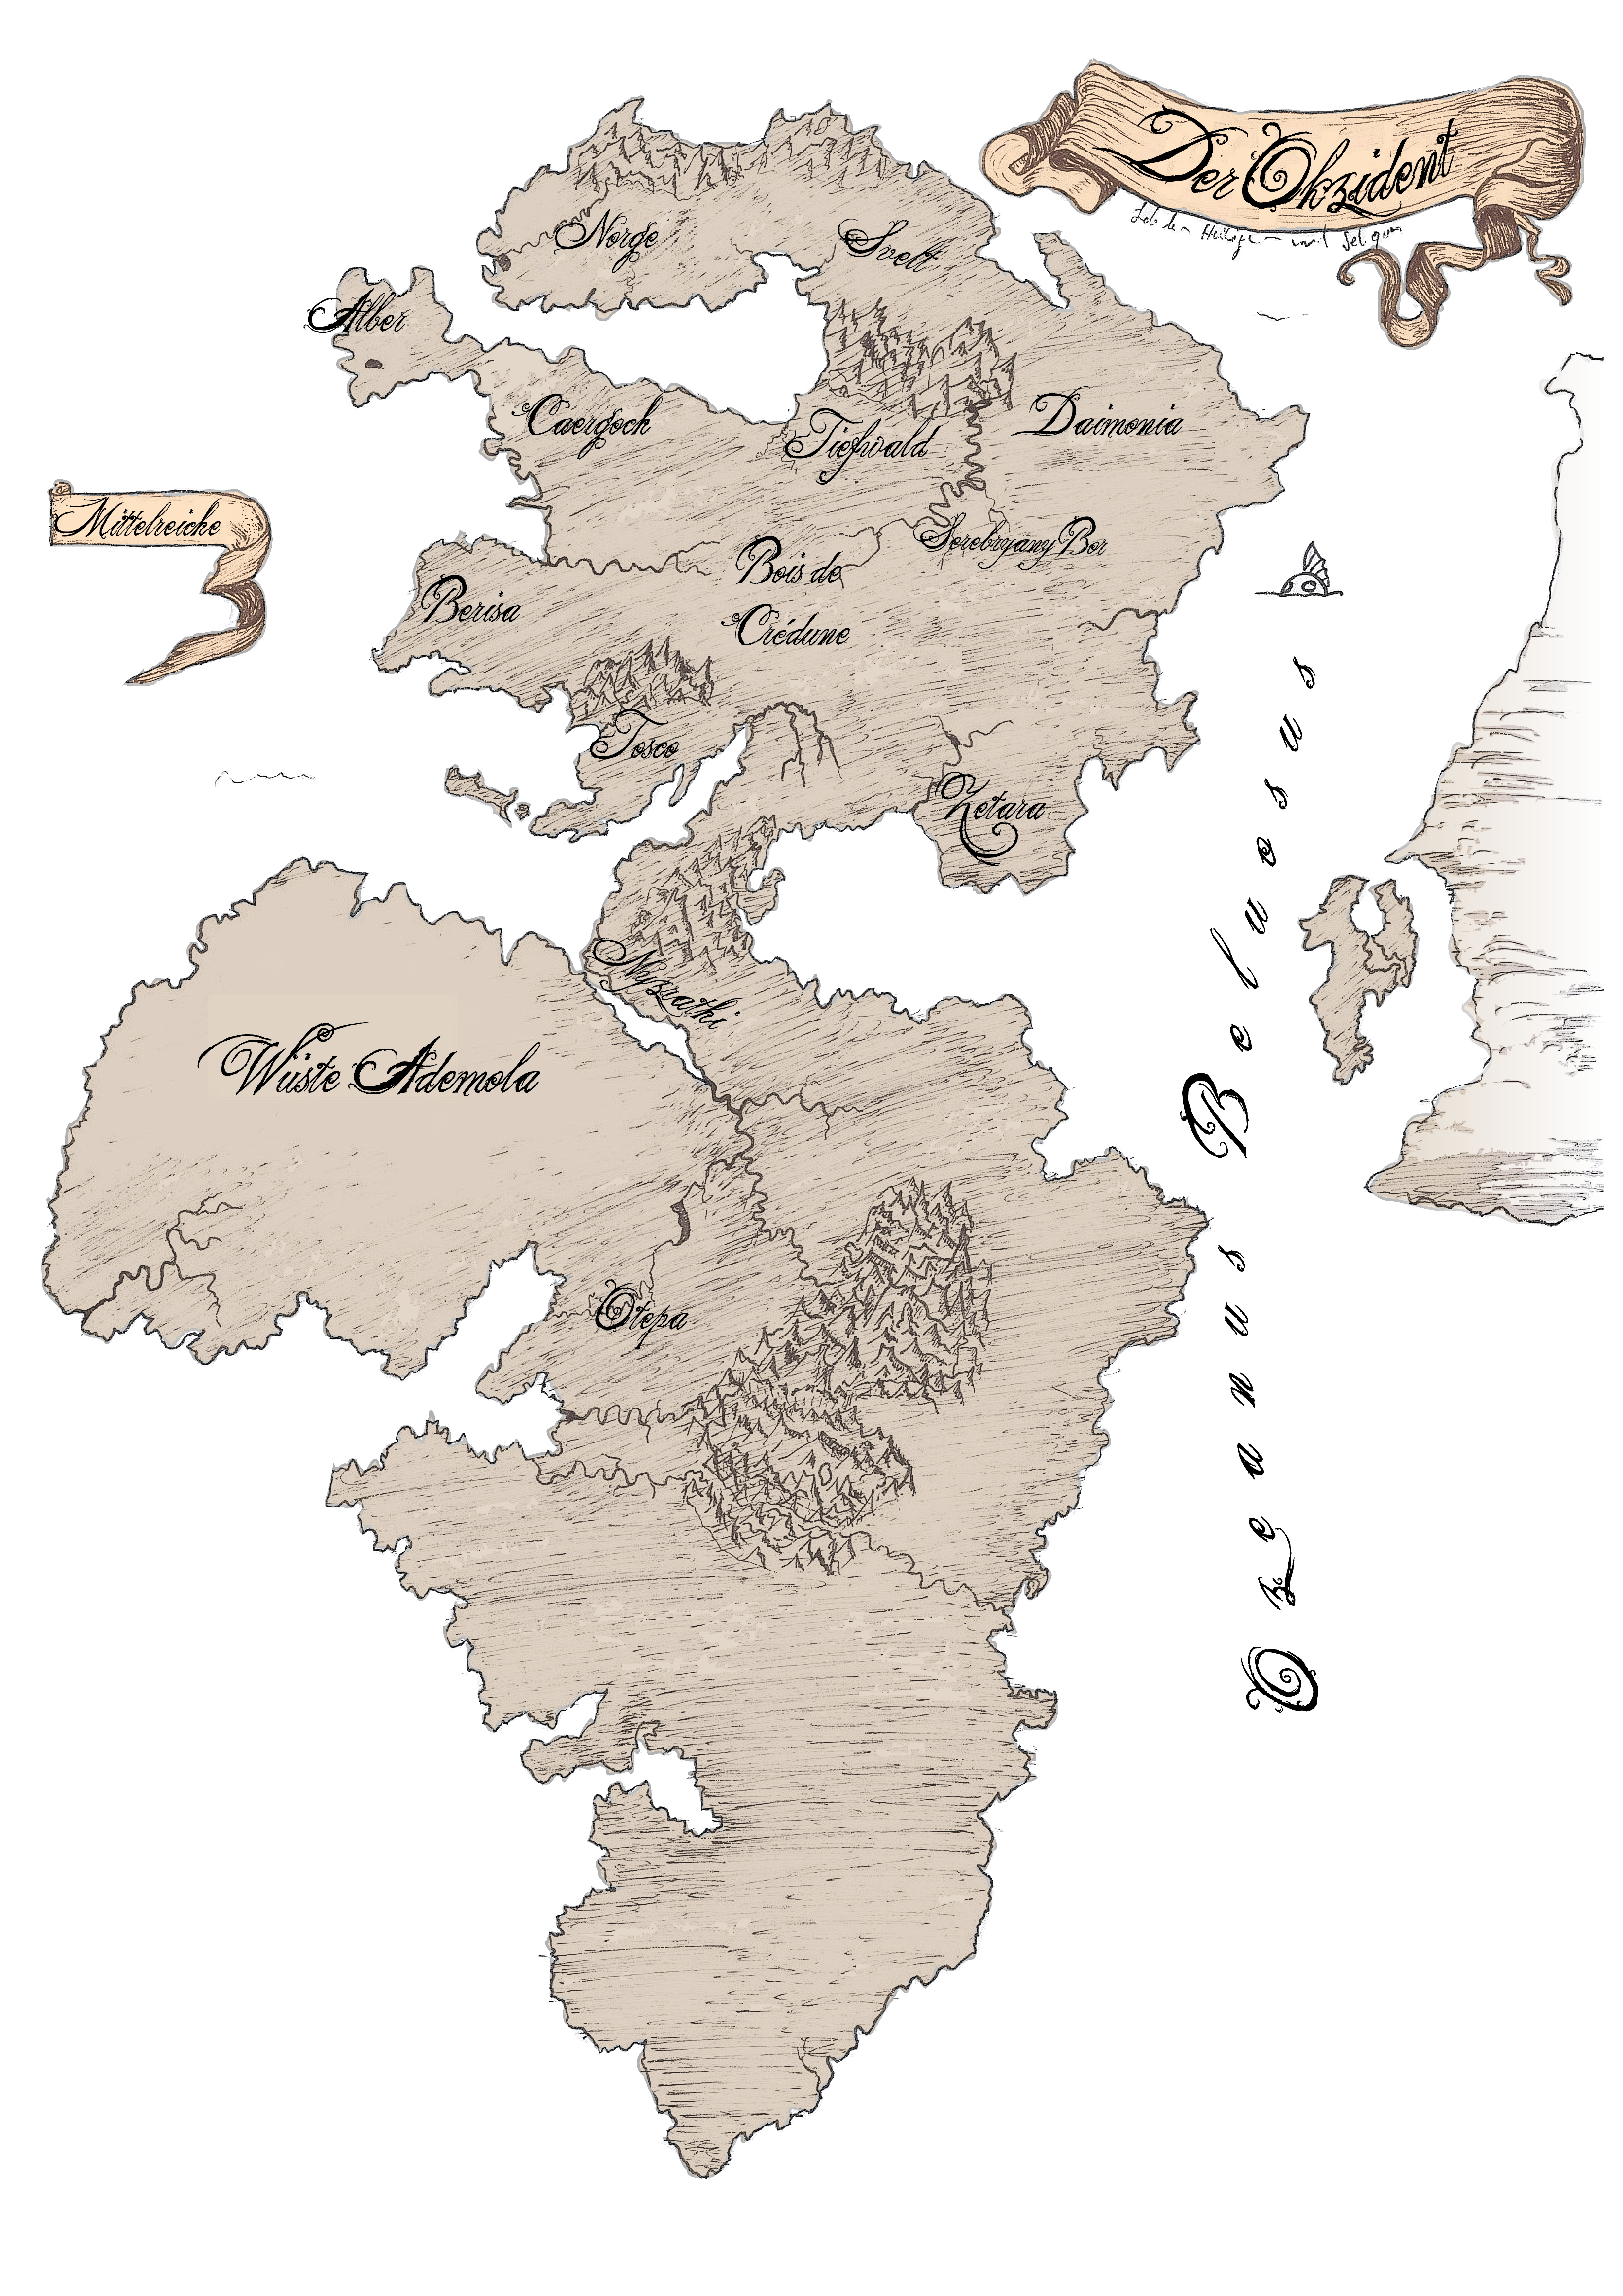
\includegraphics[width=0.9\textwidth]{b/Weltkarte1.png}
\end{figure*}

Unter der Oberfläche von Silva existieren gewaltige Hohlräume in denen es von seltsamem Leben tummelt. Dieses verworrene System von Fluren, Schächten und Kavernen wird gemeinhin das \emph{Unterreich} genannt. Pilzwälder und leuchtende Moose dominieren die Vegetation und tauchen alles in fahles Licht. Die Tiefengnome leben bevorzugt in diesen Gegenden und fördern die Schätze des Erdreichs.



\chapter{Mittelreiche}

\section{Gesellschaft}
Die Mittelreiche (Crédune, Alber, Norge, Tiefwald, Tosco, Berisa) werden von absolutistischen Monarchen beherrscht, welche sich ihrerseits stets des Rückhalts der mächtigen Adelsräte und Familien versichern müssen. Die Provinzen Caergoch und Serebryani Bor sowie die Kolonien Übersee sind Protektorate der Mittelreiche und sind stark von deren Gesellschaftsstruktur geprägt. 


\begin{table*}
	\begin{tabular}{l}
		\hline
	\end{tabular}
	\begin{tabular}{cccccc}%
		\bfseries Tiefwald  & \bfseries Alber & \bfseries Crédune & \bfseries Tosco/Berisa &\bfseries Nordländer & \bfseries Serebryany Bor\\ 
		&&&&&\\
		\csvreader[head to column names]{b/Adelstitel.csv}{}{\TW & \AB & \BC & \TB& \NO & \SB\\}
	\end{tabular}
	\begin{tabular}{l}
		\hline
	\end{tabular}
\end{table*}

\subsection{Oberschicht}
Der hohe Adel ist zugleich der hohe Klerus, denn es wird natürlich streng darauf geachtet, dass die Macht in den Händen der edlen Familien und des reinen Bluts bleibt. Der Adel gründet seine Vormachtsstellung auf Magie, Reichtum, Gewalt und rechtliche Privilegien. Die überwiegende Mehrheit aller Magieanwender, seien es Magier, Alchemisten oder Kleriker sind adelig, denn es ist in allen Mittelreichen bei Todesstrafe verboten, ohne Lizenz Magie zu wirken, und selbstverständlich dürfen nur der Adel, die Kirchen und die magischen Gilden (die ihrerseits jeweils eine Ermächtigung durch den Adel oder Klerus benötigen) eine solche Lizenz ausstellen. Ausserdem sind viele der wichtigen magischen Universitäten nur Adeligen zugänglich.

Während ein magischer Gegenstand in der Mittelschicht ein kostbares Gut und in den Slums ein Anlass für einen Bandenkrieg ist, sind sie in den Adelshäuser im Überfluss vorhanden, ein weiterer Quell für Macht und Geld.
Magische Lichter erleuchten die Hallen, magisches Feuerwerk wird bei jeder nur erdenklichen Feier in verschwenderischem Masse gen Himmel geschickt und die Wohnorte der Adeligen sind so stark mit Bannsprüchen und Protektionszaubern belegt, dass die meisten der Festungen und Prunkbauten einen lebenden Hausgeist entwickeln.

Die Vorherrschaft des Adels gründet ausserdem in seiner militärischen Macht. Mit seinem Geld kann er Söldnerheere auf die Beine stellen und zerstörerische Zaubersprüche ergänzen ein Arsenal von magischen Schwertern und Rüstungen. Doch der eigentliche Punkt ist das Wissen um Kampfkunst und Kriegsführung. Taktische Unterweisungen gehören zu der Erziehung jedes Adeligen und in Familien ist es Sitte, die spätergeborenen Jungen in Ritterorden oder Universitäten zu stecken, damit sie der Familie möglichst viel Nutzen bringen.

\subsubsection{Magier als Machtmittel}
In drei verschiedenen Kategorien finden sich Magier zusammen: Sowohl die Kirche wie die Adelshöfe haben ihre eigenen Magier, mit den Magier-Gilden aber hat auch der Mittelstand einige Zauberer. Magier des Mittelstands verkaufen ihre Fähigkeiten meist an den Meistbietenden und machen Auftragszaubereien, wie Schutzzauber für ein Haus, oder ein Feuerwerk für den Geburtstag eines bedeutenden Händlers. Der eine oder andere schliesst sich vielleicht auch als Soldmagier einer fähigen Truppe an, obwohl dies mit erheblichem Prestigeverlust einhergeht. In jedem Fall aber liegt die Kontrolle der Magier bei den Adeligen. Es ist kaum möglich, ohne einen Adelstitel Gildenvorsteher zu werden. Ausserdem wurde ein perfider Mechanismus entwickelt, die Zauberer unter Kontrolle zu behalten:

Jeder Magier schuldet seiner Gilde ungeheure Summen. Ein Zaubereibegabter niedriger Herkunft, muss sich zuallererst in eine Gilde einkaufen, um eine Lizenz zu erhalten. Ohne diese Lizenz ist Zauberei illegal und der Anwender Freiwild. Dazu kommen Kosten für die Ausbildung, teure Bücher, Unterkunft und standesgemässe Kleidung. Wer der Gilde Geld schuldet, kann kaum durch die Ränge aufsteigen oder günstige Positionen in Forschung und Lehre erhalten. Durch fleissige Arbeit alleine können diese Schulden nicht beglichen werden, schon gar nicht, wenn für arme Leute gearbeitet wird. Einer Festanstellung an einem Adelshof, in der Kirche oder bei einer Handelscompagnie geht meistens die Übernahme der Schulden durch einen Mäzen voraus.

\subsection{Mittelschicht}
Der Mittelstand geniesst zwar nicht die rechtlichen Privilegien des Adels, im Gegensatz zu den Ärmsten hat ein Mitglied des Mittelstandes ein regelmässiges Einkommen, Arbeit und muss nicht ums tägliche Überleben kämpfen. Vermögende Handwerker, Bezirksrichter und andere höhere Beamte, Ärzte, Alchemisten, Händler und reiche Bürgersfamilien sorgen für die Veränderungen in den Städten, während die Niederen nur an die nächste Mahlzeit denken und der Adel seinen Lustbarkeiten und Intrigen frönt. Der Mittelstand ist oftmals in verschiedene Gilden, Zünfte und Stadträte verbunden. Diese Organisationen haben einen beträchtlichen Einfluss auf das alltägliche Leben in der Stadt. Es existieren sogar einige wenige Städte, die vom König mit besonderen Privilegien ausgestattet wurden und nicht von einem Adeligen regiert werden. Solche „Freie Städte“ sind meist an Knotenpunkten des Fernhandels.

%\includegraphics[width=0.35\textwidth]{b/alchemist.jpg}

\subsubsection{Alchemisten und Arkantechnicker}
Alchemisten machen hochwertige Produkte und in fast jedem Beruf findet sich etwas, das mit Alchemie veredelt werden kann. Arkantechnicker erfinden Apparate  Dies ist eine der Möglichkeiten, die einem Mittelständischen bleiben, der keine oder kaum magische Begabung hat, sich mit arkanen Wissenschaften auseinanderzusetzen, denn alle vergleichbaren Künste fallen unter das Magieverbot für Nichtadelige und Nichtgildenangehörige. Natürlich müssen auch Angehörige dieser Professionen  eine Lizenz ihrer Gilde besitzen.

\paragraph{Magistri Hortulani} Die Meister der alchemischen Gärtnerkunst sind ein Bund von Alchemisten und Botanikern, die sich zusammengetan haben um eine der interessantesten Gilden zu formen, die die Welt je gesehen hat. Die Forschungen der Gilde haben bereits Wasserbäume, Luftholz und viele grossartige Früchte und Gemüse hervorgebracht. Die allermeisten Mitglieder stehen im Sold des Adels und anderer reicher Leute, wo ihnen ein Garten und die alchemischen Gerätschaften und Substanzen zur Verfügung gestellt werden. Im Gegenzug versuchen sie alle Konkurrenten mit ihren Kreationen auszustechen. Wer kreiert die schönsten Pflanzen mit den besten Effekten?


\subsubsection{Handelsconsortien und -compagnien}
Unermesslich reiche Händler, die über gewaltige Flotten von See- und Luftschiffen gebieten. Es gibt nichts womit nicht gehandelt wird: Getreide, Glas, Tabak, Kaffee, Waffen, Maschinen, Magie und Menschen.
Die besonders erfolgreichen Händler mit vielen adeligen Freunden bekommen vielleicht sogar ein vom König verbrieftes Monopol zugesprochen. Wie zum Beispiel die Compagnie Royale Crédunoise du Sud oder der tiefwäldische Kontor Stark und von Herms, die ein  Monopol auf den Handel mit Baumwolle in den südlichen Kolonien haben.
Einige Consortien leisten sich sogar ein stehendes Heer oder zumindest grosse Söldnertrupps, gewiss aber leisten sie sich mindestens einen Magier, den sie aus der Schuld seiner Gilde abgekauft haben. Für den Magier ist dies mit einem Prestigezuwachs verbunden.


\subsection{Unterschicht}
Ohne genug zu essen zu haben, ackern sich die Leibeigenen auf den Feldern und Manufakturen ihrer Besitzer kaputt. Wer Glück hat, gehört einem höheren Fürsten, der seine Ländereien mit Kämpfern und Rittern schützt. Sie leben von der Hand in den Mund.
Die Bewohner der Armutsviertel einer Stadt sind zwar insofern freier als dass ihr eigenes Leben ihnen selbst gehört, werden aber noch stärker von Hunger und Gewalt geplagt, als jene auf dem Land. Wer nicht bei einem Handwerker oder bei einer reicheren Familie eingestellt wird, ist in den Slums Freiwild. Diebesbanden liefern sich Gefechte, Schutzgelder werden erpresst und Leute werden in der Dunkelheit niedergestochen und bis auf die Haut bestohlen. Bettler und verhungernde oder dahinsiechende Kreaturen liegen auf der Strasse, - oder besser – auf dem knietiefen Morast, der in diesen Vierteln als Strasse gilt.

Neben diesen Ärmsten der Armen, die den Grossteil der Bevölkerung ausmachen, gehören natürlich alle Handwerker und sonstigen Arbeiter wie Schiffsleute, Soldaten und Söldner, freie Bauern und Quacksalber zu diesem Stand. Handwerksgesellen, Mönche und Söldner auf der Strasse, die an keinem Ort zu Hause sind und von Arbeit zu Arbeit weiterreisen, nennen sich Reysvolk. Der Begriff ist nicht zu verwechseln mit Zigeuner und anderen Vogelfreien, denn bei den Reysenden handelt es sich um freie Männer und Frauen, wenigstens dem Namen nach.

%\includegraphics[width=0.45\textwidth]{b/Soeldner}

\subsubsection{Söldner, Kopfgeldjäger und Freibeuter} Freischaffende Kämpfer, die sich für gutes Geld in den unzähligen Rangeleien zwischen den Adelshäusern als Leibwächter, Wachen, Kriegstruppen und Mörder anstellen lassen, aber auch als Bestienjäger und Schatzsucher. Auch verarmte Adelige finden hier Zuflucht. In diesem Menschenschlag sind neben der Kirche der Heiligen auch noch viele Mysterienkulte und abergläubische Sagen verbreitet, die sich zum Ärger der Kirchen als nahezu unausrottbar erwiesen haben. Überhaupt wird unter diesen Menschen wenig nach Glaube und Herkunft gefragt, wichtig sind nur ein wacher Geist und ein geschickter Schwertarm. So kommt es, dass hier nichtlizensierte Magieanwender, Verbrecher und sogar Ketzer und Werwesen zu finden sind.
Besonders der Mysterienkult um 'den Henker, den Feilscher und den Rabenvater' stellt eine beachtliche Gewalt dar und verfügt auch über Geweihte, was einige wenige regionale Teile der Kirche bewogen hat, die drei Gestalten des Kultes als Heilige anzuerkennen. Die meisten anderen ziehen es vor, solche Geweihte als Ketzer zu verbrennen.

\paragraph{Gruppierungen} Die Kriegsknechte von Delb, die Drachentötergilde, die Gilde der starken Männer und der Söldnerbund

\section{Tiefwald}
Die Herzogtümer Tiefwalds bilden den Kern des Imperiums. Tiefwald ist ein Reich, das sich auf goldenen Zeiten zuzubewegen scheint. Aus den Kolonien fliessen, Gold und Silber in die Kassen, Sklaven und Güter aller Art auf die Märkte. Als einer der wenigen Herrscher lässt Armenius den Mittelstand am neuerworbenen Wohlstand teihaben, und schafft sich so wichtige Verbündete und Allianzpartner.



\subsubsection{Imperator Arminius und sein Gefolge}
Arminius  ist nun schon der dritte von Hohenkliff, der von den Kurfürsten zum  König gewählt und ein Ende ihrer Hegemonie ist nicht abzusehen, denn wie schon sein Vater und Grossvater ist Arminius ein brillianter Politiker, Herrscher und Feldherr. Nie waren die Kolonien ruhiger, der Mittelstand zufriedener und die Kirche von der Krone abhängiger. Mit der Gründung der königlichen Universität, zu der insbesondere auch Nichtadelige zugelassen sind, und an der die niederen arkanen Küste gelehrt werden, hat er allerdings die Magier sehr verärgert.
\begin{itemize}
	\item\textit{Arminius von Hohenkliff} Der Erzherzog von Tiefwald, König von ganz Tiefwald und den Kolonien Übersee, Protektor Custodias von Serebryany Bor. Ein stattlicher Mann um die vierzig, der unter seinem Vater eine umfangreiche Ausbildung genossen hatte und die Gelegenheit hatte, sich in seinen jungen Jahren die Treue der königlichen Waldläufern zu verdienen.
	\item \textit{Kurfürst Richard 'Der Dorn' von Lohzirn} Der Herzog von Lohzirn, Kommandant der königl. Waldläufer und Garde, Busenfreund von Imperator Arminius und  Geheimrat im 2. Rat ist einer der wichtigsten Männer der Welt. Seine graue Haare und sein sehr hartes Gesicht, täuschen nicht darüber hinweg, dass er sich wahrhaftig mit Leib und Seele Imperator Arminius und dem Reich verschrieben hat.
\end{itemize}

\subsubsection{Die Kirche}

Im Herrschaftsgebiet des tiefwäldischen Kaisers werden beide Kirchenlehren befolgt: Die Tiefwäldische Kirche der Einheit Gottes Kirche der Heiligen (reformiert) in Tiefwald und Übersee und Kirche der Einheit Gottes in Serebryany Bor.
%BASTIAN SCHNEEBEERE
%\begin{itemize}
%	\item\textit{Kardinal Bastian Schneebeere} Er ist reich und mächtig. Wieso sollte er sich also etwas vorschreiben lassen. Wenn er gerne kleine Mädchen hat, kann er diese auch kriegen. In der Unterschicht gibt es ja genug, selbst welche die sowieso ausgesetzt wurden. Aber diese erwecken einfach nicht seinen Jagdinstinkt. Er findet es viel stimulierender, wenn er ein Mädchen nicht so einfach kriegt und dieses sich noch wehrt bis am Schluss. Er hat schon zahlreiche Opfer, auch aus der Oberschicht, missbraucht.
%	Ausserdem haben es ihm auch die dunklen Künste sehr angetan. Er praktiziert sie natürlich nicht selber, aber er hegt engen Kontakt. Immerhin braucht er diese um in seinem Alter noch im Bett mitzuhalten (den Gerüchten nach, lässt er sich manchmal sogar besetzen, um richtig die Sau rauszulassen).
%	Die Inquisition in Tiefwald würde ihm natürlich ein Dorn im Auge sein und somit ist sie das Einzige, das er fürchtet.
%\end{itemize}

\subsubsection{Rat der Adelshäuser}
Der Rat der Adelshäuser wählt den Imperator aus ihren Reihen. Er hat jedoch mehr repräsentative Funktion und bei diesen Wahlen gibt es kaum Überraschungen. Die wichtigen Entscheidungen werden im Königlichen Geheimrat gefällt.

\paragraph{Königlicher Geheimrat} Auch genannt der zweite Rat. Ein Geheimrat von hohen Adeligen der Hauptstadt Tiefwalds, die meist unter dem Vorsitz des Königs über die wichtigsten Angelegenheiten des Reiches, insbesondere über den Erlass von Verordnungen, Beschluss fassen. Die letzte Instanz ist der Imperator persönlich. Auch die Erlaubnis zu heiklen Ermordungen durch eines der „Staatskabinette für interne Angelegenheiten“ fällt unter die Verantwortung dieses Rates. Diese Assassinengilden von Tiefwald sind fürchterlich verzankt und im ewigen Wettstreit.




\subsubsection{Die Institutionen Tiefwalds}

\paragraph{Akademie für Alchemie und Technick} Die Königlich-Tiefwäldische Akademie für Alchemie und Technick versucht die klügsten Köpfe für den wissenschaftlichen Fortschritt des Reiches zu gewinnen. Flugmaschinenkonstruktion, Zauberschmieden, Chirurgie und thaumatische Waffentechnick sind Vorlesungen, die man dort besuchen kann. Unter den Adeligen ist die Schule nicht angesehen, weshalb hier vor allem reiche Bürgersprosse mit leichter Magiebegabung studieren. Die Akademie hat an verschiedenen Universitäten in ganz Tiefwald neue Fakultäten begründet.

\paragraph{Komissariat für Magische Verbrechen} In Tiefwald obliegt die Aufgabe, unlizensierte Magieanwender zu finden, dem gnadenlosen Komissariat für magische Verbrechen. Die Kirchen stören sich sehr daran, dass es ihnen nicht gestattet ist, diese Aufgabe auszuführen wie in den Nachbarländern. Die Magiergilden dagegen befürworten diese staatliche Institution.


%KOENIGLICHE POST

%\paragraph{Königliche Post}

\paragraph{Königliche Waldläufer} Diese Elitesoldaten sind dem Imperator treu ergeben, hat er doch seine Karriere als Offizier bei den Waldläufern begonnen. Nicht nur sind die Waldläufer hervorragende Krieger und Leibwachen, sie dienen auch als Augen und Ohren des Imperators und bewachen die Wälder Tiefwalds.

\paragraph{Magiergilden} Jede grössere Stadt hat mindestens eine Magiergilde, manche sogar mehrere. Die mächtigste Gilde ist sicherlich diejenige von Tiefwald-Stadt, die sich auch gerne als die Dachorganisation aufspielt.
\begin{itemize}
	\item\textit{Convocata Mathilde von Lach} Als sie klein warm, hat Hofmagister Magnus Stefan Freudenbein sie aufgenommen und ihr Magie beigebracht. Sie hat ihn aber schnell überflügelt in fast allen Kategorien (ausser Freudenbeins Spezialgebiete, in denen er unschlagbar ist) und ist heute ohne zweifel die mächtigste Magierin in Tiefwald-Stadt (allerdings haben mächtige Magier die Tendenz sich in die Einsamkeit zurückzuziehen und es ist deshalb durchaus möglich, dass in den Wäldern von Tiefwald noch viel mächtigere Magier hausen).Sie ist Gildenherrin (Convocata) der Magier-Gilde und Rektorin der Magie-Universität und hat einen Sitz im 2. Rat
	Selbst sie kann höchstens raten wie alt Stefan Freudenbein wirklich ist.
\end{itemize}



\paragraph{Spitzelnetzwerk} Wenn ein Imperium funktionieren soll, wie ein gut geschmiertes Räderwerk, müssen die Herrschenden informiert sein. Dazu bespitzeln sich alle gegenseitig.
\begin{itemize}
	\item\textit{Ainbald der Informant} Es gibt scheinbar nichts, das er nicht weiss. Aber er ist nicht leicht zu finden. Tatsache ist, meistens findet er seine Kunden. Alles was einem übrigbleibt, wenn man ihn braucht, ist dies bekannt zu machen, so dass er Kontakt aufnimmt. Aber nur weil man mit ihm in Kontakt getreten ist, heisst das noch nicht, dass man seine Information wirklich bekommt. Er ist nicht an Gold interessiert und lässt sich oft ausgefallene Zahlungsmethoden einfallen.
	Wenn man ihn im Nachhinein zu beschreiben versucht, stellt man fest, dass man sich nur noch schwer an bestimmte Merkmale seines Äusseren erinnern kann. Ausserdem wird er auch nicht auf arkanen Überwachungsgeräten aufgezeichnet und seine Spuren verwischen sich von selbst.
\end{itemize}

\subsection{Serebryany Bor (Protektorat)}
Die Provinz Serebryany Bor wird von tyrannischen Kleinfürsten regiert. Und nicht nur in den Wäldern treiben sich, bedingt durch die unmittelbare Nähe zu Daemonia widernatürliche Gestalten herum: Von manch einem Landherr heisst es, er sei ein Vampir, der sich in der Nacht aus seinem Sarg erhebt und sich über zarte Jungfrauen hermacht. Auch der gelegentliche Werwolf wird dort gesichtet und dann vom Pöbel zum Scheiterhaufen gebracht, auch wenn es der herzensgute Dorfpfarrer sein sollte, der zu viele Haare hat. Der Menschenschlag dort ist misstrauisch, gemein und hinterhältig.

%Tiefwald-Stadt
\subsection{Tiefwald-Stadt}

Die Hauptstadt von Tiefwald.

\subsubsection{Stadtrat Tiefwald-Stadt} Obwohl der Stadtrat keine formalen Befugnisse zur Regierung des Reiches hat, werden seine Mitglieder oft vom Imperator konsultiert. Damit erhält prinzipiell auch der bürgerliche Stand eine Stimme. Neben den Patriziergeschlechtern erhalten der Rektor der königl. Akademie für Alchemie und Technick sowie die Convocata der Magiergilde einen zugesicherten Platz im Stadtradt.

\subsubsection{Die Burgstadt}
Im oberen Teil der Stadt wohnen die reichsten Patrizierfamilien und Adeligen. Jede Adelsfamilie, die etwas zählt und ihren Einfluss bei Hof gelten machen will, unterhält in der Burgstadt einen unerhört teuren Prunkbau. Die Botschaften fremder Staaten sind ebenfalls hier zu finden. Läden verkaufen Luxusartikel, seltene Kolonialwaren und teuerste Stoffe aus aller Welt. Eine dicke aber altertümliche Mauer geht von der Festung aus um die Burgstadt und zeugt davon, dass dies der älteste Teil der Stadt ist.

\paragraph{Festung Nydegg} Die angeblich mächtigste Festung der Welt, türmt hoch in den Himmel. An den Flanken sind Andockstellen für Luftschiffe, so dass die Allerhöchsten gar nicht mit der Stadt in Berührung kommen müssen. Die Festung ist die Residenz des Hochkönigs Arminius, seiner Familie und seiner engsten Vertrauten, sowie den Höflingen.

\paragraph{Königshof} Der Hof des Königs hat ein riesiges Eigenleben entwickelt. Der gewaltige Reichtum, der in Tiefwald-Stadt kumuliert ist, führt dazu, dass prunkvolle Feste und Bälle veranstaltet werden, an denen exotischen und kostspieligen Genüssen gefrönt wird. Es ist ein Sehen und Gesehenwerden, an dem der Imperator selbst äusserst selten teilnimmt. Nichtsdestotrotz werden hier wichtige Netzwerke gepflegt und Päkte geschlossen.
\begin{itemize}
	\item\textit{Magister Magnus Stefan Freudenbein}, Hofmagier
	Keiner weiss wie alt der Hofmagier wirklich ist. Er scheint genau so alt zu sein wie die Festung selbst und dennoch völlig nutzlos. Er hat ein Loch in der Mauer kreiert, das er konstant durch eine Illusion versteckt hält (mit Hilfe eines Artefakts). Diesen Durchgang nutzt er um insgeheim Frauen, vor allem Prostituierte, in die Festung zu schmuggeln, wo er ihre Dienste braucht und sie danach den Geheimgang vergessen lässt. Er kennt nur Magie, die ihm für seine Freuden und Lüste nützlich sind, in diesen ist er jedoch unübertroffen.
\end{itemize}

\paragraph{Zytglogge} Das Torhaus Zytglogge trennt Burg- und Mittelstadt und beherbergt verschiedenste magische Apparate, die - zusammen mit ihren Gegenstücken in der Festung - die Burgstadt mit einem Schutzschirm aus diversen Zaubern überziehen. Ausserdem prangt eine riesige Uhr an der Fassade.

\subsubsection{Mittelstadt}

\paragraph{Käfigturm} Der Käfigturm trennt die Mittelstadt von der Vorstadt. Der Käfigturm ist ein dicker, etwa sieben Stockwerke hoher Turm. Unten ist das Tor mit Fallgattern, daneben eine breite Tür, durch die man in den Turm kommt. Über dem Tor steht eine gewaltige \emph{Statue des heiligen Christoffel}, von der man sagt, sie sei ein Golem, der bei Belagerung der Stadt zum Leben erwacht, um die Stadt zu verteidigen. Der Käfigturm ist über und über mit Käfigen bedeckt, die an schweren Ketten an der Aussenwand herabhangen. Sie sind in der Regel leer, weil heutzutage ja bessergestellte Anwohner da sind, aber die Drohung ist unverhohlen. Auch die Inneren Zellen sind nur kurz belegt, das eigenetliche Gefängnis befindet sich ausserhalb der Mauern.
Im Turm hat der Major der Grenzwache sein Büro und die höheren Strafverfolgungsbehörden der Stadt benutzen den Turm, um Verdächtige abzuklären, bevor sie dann in ein Gefängnis einer Behörde verschwinden (oder für immer).
\begin{itemize}
	\item \textit{Meister Gallus} ist der Folterknecht, der im Turm seine Festanstellung hat. Er ist ein fetter, schwitzender Glatzkopf mit einer Lederschürze, auf der verschiedenste getrocknete Körperflüssigkeiten sind. Die Schürze beherbergt einen Haufen Zangen, Klemmen und Messer, sowie ein Notizbuch, in dem er seine Arbeit säuberlich dokumentiert.
\end{itemize}

\subsection{Karlsbruck}
Eine grosse Stadt im Osten von Tiefwald. Der Fluss Siebenlauf teilt die Stadt entzwei. Verlässt man die Stadt in östlicher Richtung, betritt man das Protektorat Serebryany Bor. Karlsbruck hat eine grosse Garnison, die in den Wäldern und Dörfer von Serebryany Bor den Frieden wahren.




%ALBER
\section{Alber}
\paragraph{Herrscher} Bartholomeus II, King of Alber, Supreme Ruler of the Empire
\paragraph{Staatskirche} Kirche von Alber
\subsection{Caergoch (Protektorat)}
Ein Provinznest bewohnt von Hinterweltlern mit einer Sprache, die niemand versteht und die sich mit Waid bemalen und unzivilisierten Bräuchen und Göttern anhängen. Alle paar Generationen wehren sie sich wieder gegen die Herrschaft durch Alber. Es wird viel Blut vergossen und je nach Ausgang werden einige Grenzen etwas verschoben, die Tributzahlungen werden erhöht oder gesenkt und einige Clanführer erhalten einige Sonderrechte oder verlieren sie wieder an Albers Adelige.

\subsubsection{Institutionen}
\paragraph{Arrows of Light} Ein weissmagischer Orden, der Schwarzmagier und Nichtlizensierte jagt. Der Orden grenzt sich stark von der Kirche ab.

%ALBYRION
\subsection{Albyrion}
Die Hauptstadt von Alber.

\begin{table*}
	\centering
	\begin{tabular}{l}
		\hline
	\end{tabular}
	\begin{tabularx}{\textwidth}{cXcXcX}%
		\bfseries W100  & \bfseries Männername & \bfseries W100  & \bfseries Männername & \bfseries W100 & \bfseries Frauenname\\ 
		&&&&&\\
		\csvreader[head to column names]{b/Vornamen_m.csv}{}{\W & \Mann &\w& \mann & \ww & \frau\\}
	\end{tabularx}
	{Häufigste Namen 1411 bis 1497, zusammengestellt von beliebte-vornamen.de}
	\begin{tabular}{l}
		\hline
	\end{tabular}
\end{table*}

\chapter{Nyzrathi, Zetara und die Freistaaten}
Nur wenige Landstriche und Städte im Okzident vermögen sich dem Zugriff der grossen Monarchien zu entziehen. Zu nennen sind hier der Stadtstaat Nyzrathi, der Städtebund Zetara und die von Piraten beherrschten Freistaaten zwischen der Ademola und dem Beris-Meer.

\section{Republik Nyzrathi}
Die Stadt Nyzrathi ist eine handelstechnisch günstig im Nyzdelta gelegene Metropole. Nyzrathi ist wahrscheinlich die vielfältigste und offenste Stadt der Welt. Als Drehpunkt des Fernhandels in alle Richtungen, hat Nyzrathi einen gewaltigen Reichtum erworben und dank seines aussergewöhnlichen Regierungssystems kam dieser Reichtum einer breiteren Schicht zugute als dies anderswo der Fall wäre.

Das Herrschaftsgebiet der Republik Nyzrathi erstreckt sich über einige benachbarte Städte, die unter der Herrschaft des Dogen und des Stadtrats von Nyzrathi stehen sowie einige weitere Städte, die auf dem Papier unabhängig sind, aber von Marionetten des Hexen-Rates regiert werden. Dieses beachtliche Gebiet grenzt im Norden an Tosco und den Städtebund Zetara, im Süden an die Wälder von Otepa und im Westen an die Freistaaten und die Wüste Ademola.

Jede Religion des Okzidents hat im Laufe der Jahrhunderte in Nyzrathi eine Heimat gefunden. Der Heilige Geist, die alten Götter und die Naturgeister werden alle angebetet und es finden sich entsprechende Tempel in der ganzen Stadt. Meist werden die Texte liberaler ausgelegt, als das in den Herkunftsländern der Fall ist und wenn beispielsweise der Bischof von Nyzrathi zu einer Konferenz in Berisa reist, wird man seine Ansichten dort als extrem ansehen.

Die Politik in Nyzrathi ist das verworrenste Netz von Beziehungen, Fehden, Interessengruppierungen, Räten und Bestechung, das je von Menschen geschaffen werden kann.

\subsubsection{Rat der Weisen Frauen (Hexenrat)} Der Hexenrat ist die Antwort auf die Herausforderung, einen Stadtstaat zu regieren, der eine unüberschaubare Zahl von Ethnien, Religionen und Interessensgruppen beherbergt. Die Weisen Frauen sind Vertreterinnen dieser Gruppen - Priesterinnen, Adelige, Kräuterfrauen, Kapitäninnen und zaubermächtige Hexen. Durch ein komplexes Netz zwischenmenschlicher Beziehungen nehmen die Weisen Frauen Einfluss auf jeder Ebene der Gemeinschaft. Sie gelten als unbestechlich und gerecht, wenn auch manchmal hart.

Der Hexenrat verfügt Gesetze für die Stadt und Republik Nyzrathi (eine Bezeichnung, welche die zugewandten Orte einschliesst) und ernennt Statthalter, Hauptmänner der Wache und Richter.
\begin{itemize}
	\item\textit{Nesmeralda} Niemand weiss, wie alt Nesmaralda ist. Andere Hexen sagen, dass Nesmeralda schon graue Haare hatte, als sie dem Rat vor zwanzig Jahren beitraten. Und während sie selbst graue Haare bekamen, schien Nesmeralda kein bisschen an Kraft zu verlieren. Man sagt, dass sie mächtige Zauberei beherrsche und nicht altere, dass sie vor langer Zeit barfuss aus dem fernen Serebryany Bor nach Nyzrathi kam und den Aufstieg der Hexen in Gang setzte. Fest steht, dass sie die grösste Fraktion im Hexenrat führt und ihr Wort ein Gewicht hat, dass man sonst nur den mächtigsten Fürsten der Welt beimessen würde.
\end{itemize}

\subsubsection{Doge und die Adelshäuser} Der Doge regierte ursprünglich als König über Nyzrathi, aber die Position hat im Laufe der letzten 150 Jahre massiv an Einfluss verloren und heute hat der Doge kaum mehr Einfluss auf die Gesetzgebung. Nur wenn seine Unterschrift vonnöten ist oder ein veraltetes Gesetz Anwendung findet, gelingt es dem Dogen, dem Hexenrat Widerstand zu bieten. Zudem kann er als oberster Richter Einfluss nehmen und er hat die Befugnis einige Steuern festzusetzen und einzutreiben. Zudem verfügen die Familie des Dogen sowie die verbündeten Häuser eine beachtliche Privatarmeen.

\begin{itemize}
	\item\textit{Der Doge Carlos lo Aziz} ist unfähig und hat es nur seiner Mutter und seinen Kindern zu verdanken, das die Familie Lo Aziz noch einen Teil der Macht hat.
	\item\textit{Angelo lo Aziz}, der Sohn des Dogen, ist ungebrochen populär bei vielen Bevölkerungsgruppen wie z.B. den konservativen, frauenfeindlichen Kabb'lern und Priestern, den älteren Adelsgeschlechtern und den Monarchisten im Volk.
	\item\textit{Catharina lo Aziz}, die wunderschöne Schwester von Angelo, ist eine begabte Magierin und bereitet sich vor, den Sitz ihrer Grossmutter im Hexenrat zu übernehmen.
	\item\textit{Magaly lo Bairdyz},  die Mutter des Dogen,  vertritt die Familie im Hexenrat. obwohl ihr der grösste Teil der Weisen Frauen ablehnend gegenübersteht, kann sie durch ihre raffinierten Schachzüge trotzdem etwas erreichen.
\end{itemize}

\subsection{Stadt Nyzrathi}
\subsubsection{Distrikte von Nyzrathi} Die verschiedenen Distrikte der Stadt dürfen sich innerhalb von bestimmten Grenzen selbst organisieren, solang die übergeordneten Gesetze eingehaltet werden. Zwischen den Distrikten herrscht ein (meist freundlicher) Wettbewerb. Die grösseren Distrikte wie der Universitätsdistrikt, Markt und Hafen sind sehr multikulturell und werden oft von wirtschaftlichen Interessen der Gilden und Zünfte beherrscht. Die Gilden und Zünfte schicken ihre Vertreter(-innen) sowohl zum Dogen wie auch in den Rat der Hexen. Eine Magiergilde wie in den Mittelreichen gibt es nicht, da Nyzrathi keine Lizenzpflicht für Magiekundige kennt. Stattdessen schliessen sich Zauberwirker anderen Gilden oder Zünften an oder schliessen sich zu Schulen zusammen. Jeder Stadtteil hat ihre eigenen Gilden, die sich wiederum einer Dachorganisation anschliessen.

\subsubsection{Wichtige Bevölkerungsgruppen}
\paragraph{Die Kabb'ler} In Nyzrathi lebt die grösste Gemeinschaft von Kabb'ler der Welt. Viele berühmte Kabb'ler lehren an den Schulen und der Universität und auch in den Gilden finden sich einflussreiche Kabb'ler - alles Positionen, die ihnen aufgrund von religiösen Vorurteilen in anderen Ländern oft verwehrt sind. Die Kabb'ler sind jedoch alles eine einheitliche Gruppe. Konservative Kabb'ler empfinden den Hexenrat und das damit einhergehende Matriarchat als gotteslästerlich und versuchen die Position des Dogen zu stärken, gleichzeitig sind einige Maharati (die weiblichen Priesterinnen) sowie Magierinnen und Ärztinnen  Mitglied in ebendiesem Gremium. Konflikte zwischen Gruppen in Nyzrathi sind oft davon geprägt, dass die verschiedenen Gruppen unterschiedlichen Ethnien angehören. Kabb'ler stellen hier eine Ausnahme dar, da sie Konflikte mit anderen Kabb'lern viel verbissener und kleinlicher führen, als mit irgendwem sonst.

\paragraph{Ougdou} Wie die Stadt Nyzrathi selbst ein Gemisch verschiedener Menschen ist, ist Ougdou ein Amalgam verschiedener Religionen. Die meisten Menschen in Nyzrathi folgen dieser Lehre und entsprechend ist ihr Einfluss auf das Erscheinen und den Alltag der Stadt sehr gross. In den Gassen riecht es nach den Gewürzopfern, die Gläubige den Loas darbringen. An Türen hängen rituelle Schutzsymbole. An Feiertagen sind die Strassen voller Tanzenden. Tiere werden geopfert und die Mambos sprechen in Zungen.

\paragraph{Ausländer} Viele Mittelländer leben in Nyzrathi und leben dort getreu den lehren des Heiligen Geistes. Nyzrathi verfügt über einen eigenen Bischof, der allerdings in den Kreisen der Kirche in Berisa und Tosco nur unwillig geduldet wird. Aus den Königreichen des Südens kommen mit wertvollen Gütern auch viele Menschen nach Nyzrathi.

%\subsection{Zugewandte Orte}
%Die Städte, die sich der Herrschaft des Dogen und des Hexenrates in unterschiedlichem Masse unterworfen haben, werden die zugewandten Orte genannt.

%ZETARA
%\subsection{Zetara}
%
%	
%\subsubsection{Confederatio Urbium Liberarum Zetarum}
%
%
%\paragraph{Schmieden von Zetara}

%==================================================================================================


\chapter{Kosmologie \& Religion}
%		\item Vitalitas, Wachstum als Prinzip des Lebens
%		\item Morbus, Verderben als Prinzip des Sterbens

	Religionen werden insbesondere auch zur Beantwortung kosmologische Fragen herangezogen, also der Frage wie die Welt beschaffen und entstanden ist. Auch die Frage, wie übernatürliche Kräfte wirken, fällt meist in den Bereich der Religionen.
	Im folgenden sollen verbreitete Grundmodelle vorgestellt werden.
	
	Im Okzident am meisten verbreitet ist das Sphärenmodell, dessen Grundzüge vom Heiligen Thomas entwickelt wurde. Es trennt zwischen göttlichem Wunderwirken und der Magie, die weiter verschiedene Quellen hat, die alle als Sphären um die materielle Welt angelegt sind. Mehr dazu unter der Religion des Heiligen Geistes.
	
	Bei vielen älteren Religionen, insbesondere verschiedenen Natur- und Schamanentraditionen gibt es keine klare Trennung zwischen Geist und Materie. Vielmehr hat jedes Wesen eine duale Natur, also gleichzeitig eine Erscheinung in der Geisterwelt und in der materiellen Welt. Die Stärke und Sichtbarkeit des Wesens in den beiden Welten kann dabei sehr verschieden sein. Während in den Mittelreichen die Verehrung aller Wesen ausser Gott und den mit ihm vereinigten Heiligen als Götzenkult abgelehnt wird, ist die Verehrung von Nymphen, Dryaden, Ahnen- und Tiergeistern sowie minderen Göttern z.B. in der schamanistischen Tradition des Königreichs Otepa viel wichtiger als jene des Schöpfergottes Ologun, der sich nicht mehr in den Lauf der Dinge einmischt. Die alten druidischen Religionen im Norden glauben an mehrere Götter, die die Welt zusammen mit ihren Gegnern, den Riesen, geschaffen haben und sie pflegen den Kontakt zu Naturgeistern und Elemntaren.

\begin{table}[htpb]
	\begin{commentbox}{Bemerkungen zur Weltordnung}
		Im Gegensatz zu D\&D oder DSA möchte ich keine 'offizielle' oder bevorzugte Kosmologie, sondern mehrere gleichberechtigte. Wer mehr zu den Religionen des Südkontinents erfinden will, soll sich doch von der Wikipediaseite 'Afrikanische Kosmogonie' inspirieren lassen.
		
		Dem aufmerksamen Leser werden die Inspirationsquellen für die Religionen Silvas sicher nicht entgehen:
		\begin{itemize}
			\item \emph{Heiliger Geist} Christentum
			\item \emph{Kabb'l} kabbalistisches Judentum
			\item \emph{Ougdou} Voodoo
			\item \emph{Otepa} Yoruba (Afrikanisches Volk)
		\end{itemize}
	\end{commentbox}
\end{table}
	
	

	
\section{Religionen}

 \subsection{Der Heilige Geist}
 Nach den Magierkriegen verbreitete sich der Glaube an den heiligen Geist sehr rasch.
 
	\subsubsection{Thaumaturgie \& Magie}
	Im Glauben an den Heiligen Geist ist die Unterscheidung zwischen Thaumaturgie, also durch Menschen vermitteltes göttliches Wirken und der Zauberei sehr wichtig. Nur die Thaumaturgie, das Wunderwirken, kann tatsächlich die Naturgesetze überwinden. Wunder geschehen, wenn der Glaube eines Gläubigen so tief ist, dass die Anwesenheit des Heiligen Geistes die Schöpfung auf übernatürliche Weise verändert. Zauberei wird auch als präternatürlich (neben der Natur) bezeichnet. Im Gegensatz zu übernatürlichen Phänomenen ist Magie vielleicht nicht verstanden, aber grundsätzlich erklärbar.
	Zauberei folgt ihren eigenen Regeln und erschliesst sich einem wissenschaftlichen Geist. Die Quelle ihrer Kraft, der Aether, kann mit Messgeräten erfasst und für arkantechnische Zwecke gebraucht werden. Dagegen entspringt die Kraft der Thaumaturgen ihrem Glauben und einer tiefen philosophischen Überzeugung.
	
	\subsubsection{Pilgerwege und die Weihe}
	Überall verstreut auf Silva gibt es Orte thaumaturgischer Macht, genannt Sedoi (singular Sedos). Diese Orte gelten üblicherweise als Heiligtümer der lokalen Kirchen und werden von diesen wie ein Augapfel gehütet und nach Möglichkeit geheim gehalten. Oft wird ein Kloster oder ein Tempel an der Stelle gebaut. Es heisst, diese Wege seien Pfade, auf denen die Heiligen gewandelt und gewirkt haben. Die Pilgerwege sind der Schlüssel zu den Geweihten (als Synonym für Thaumaturgen): Ein Mönch, der von seinen Vorgesetzten als würdig erachtet wird, darf den Pilgerweg bereisen. Am Antritt der Reise steht oft ein mehrtägiges Fasten und Beten, das den Gläubigen in die richtige geistige Verfassung bringen soll.
	
	Jeder Pilgerweg besteht aus einem oder mehreren Sedoi. An jedem Sedos, typischerweise duch einen Altar oder einen grob behauenen Stein gekennzeichnet, wird gebetet und meditiert. Bei den allermeisten Probanden hat die Zeremonie keine weiteren Auswirkungen. Einige wenige jedoch erleiden plötzliche Schmerzen, Verlust von Sehkraft, Lähmungen von Gliedern. Diese Gebrechen nehmen von Station zu Station zu, bis sie mit der Vollendung des Pilgerweges plötzlich verschwinden und der Proband seine gewonnenen thaumaturgischen Kräfte wahrnimmt. Bei denjenigen, die die Torturen davon abhalten, den Weg zu beenden, ebben die Qualen langsam innerhalb von Tagen, Wochen oder Monaten ab. Generell sind längere Wege riskanter und schwerer zu begehen, bringen aber auch stärkere Kräfte mit sich. Die genaue Form der erhaltenen Kräfte hangen vom Charakter des Probanden, aber auch vom Charakter des Heiligen ab, der den Weg beschritten hat.
	
	Generell sind Geweihte unglaublich geachtet und ihr Status relativiert ihre Herkunft: Geweihe von niederer Herkunft können bis in hohe Ränge aufsteigen, und Geweihte adeliger Herkunft fühlen sich ihrem Glauben stärker verbunden als ihrer Familie. Tatsächlich gibt es aber viel zuwenige Geweihte, um einen wirklichen Unterschied zu machen. Die Mehrheit aller Kirchenangehörigen sind gewöhnliche Mönche und Nonnen, Dorfpriester und sowie einige Tempelritter von niederem Adel.
	
	\subsubsection{Die Kirchen}
	Die (reformierte) Kirche der Heiligen wird in Alber, Norge und Tiefwald verehrt, die Lehre der (orthodoxen) Kirche der Einheit Gottes wird in allen anderen nichtheidnischen Ländern befolgt.
	
	Die Kirchen verehren die Heiligen als Ausdruck der Kraft des einen Gottes und verfügt über die Geweihten, Mönche und Priester mit mystischen Fähigkeiten. Die jeweiligen Kirchen haben zwar einen gemeinsamen theologischen Überbau, aber die Orden der verschiedenen Heiligen haben jeweils ihre eigenen Streitkräfte und ihre eigenen Motive, die sich zum Teil stark unterscheiden können. Auch sehr unterschiedlich ist die Stärke der Verbandelung von Adelshäusern und Kirchen.
	\paragraph{Kirchliche Institutionen} Hospitaliterorden, die Templer zur leeren Hand, Liga zur Verteidigung des Glaubens, Inquisition Royale Crédunnoise
	
	
%		Auch wenn viele andere Modelle existieren, die Kosmologie des hl. Thomas ist sicher die in den Mittelreichen verbreitetste und populärste. Er ist der offizielle Kanon beider Kirchen und vieler Magieakademien und stützt sich auf die heilige Schrift. Auf die Schöpfung der Planeten und Sterne aus dem Nichts und die Trennung von Licht und Schatten (durch die Sterne) folgt die Trennung von Körper und Geist (die Thomas interpretiert als Trennung der Realwelt vom feinstofflichen Aether) und die Trennung von Himmel und Erde (interpretiert als das Gestalten des Planeten Silva). Schlussendlich folgt die Trennung von Leben und Tod, verbunden mit der Kreation der Seele und des freien Willens. Gestützt auf dieses Modell beschreibt Thomas die verschiedenen, einander durchwirkenden Ebenen:


	\begin{paperbox}{Sphärenmodell des Hl. Thomas}
		Der heilige Thomas lebte von 1498 bis 1581 und war ein Geweihter im unabhängigen Orden der Parenser. Seine Gaben umfassten Visionen, mit deren Hilfe er die kosmologische Ordnung zu ergründen suchte. Das gewonnene Wissen teilte und verfeinerte er in gelehrten Aufsätzen und Diskussionen. Er wurde von beiden Kirchen heilig gesprochen.
		
		Die Oberfläche des Planeten Silva, das Unterreich und das darunter, nahe am Planetenkern liegende Kerkerreich bilden die \emph{Materielle Sphäre}.
		
		Stark mit dem Aether verbunden sind die Sphären der Feen, die \emph{Anderswelt}, wo Zeit und Raum nach anderen Regeln spielen.
		
		Im Äther befindet sich der \emph{Abyss}, auch Hölle, wo die D\ae monen wohnen, die sich gegen Gott gewandt haben. Eine verdorbene Seele, die nicht von Gott erlöst wird, kann sich nicht aus dem Aether lösen und treibt schliesslich in den Mahlstrom des Abyss, wo sie auf Ewigkeit, versklavt und gefoltert wird.
		Die Seele der Erlösten werden von Gott aufgenommen und sind wie Er allgegenwärtig. Die gläubigsten und heiligsten Seelen dürfen dabei die Menschen in ihrem Streben nach Erlösung unterstützen, weshalb als thaumaturgische Kräfte weiterhin präsent sind.
	\end{paperbox}

	\subsection{Ketzerei und Kulte}

	Im allgemeinen Sinn wird das Wort Ketzer für alle gebraucht, die vom rechten Glauben abgefallen sind und Irrlehren verbreiten. Im besonderen meint man damit aber Menschen (und andere Wesen), die thaumaturgische Kräfte besitzen, ohne dabei aber den Lehren der Kirche zu folgen. Dies umfasst Gläubige, die nicht-santionierte Heilige anbeten (von der Kirche manchmal als Schwarze Heilige oder Unheilige bezeichnet werden) oder einer kleinen Splitterreligion angehören. Oft sind diese Gläubigen in Mysterienkulten organisiert, die sich meist durch grosse Geheimhaltung und Vorsicht vor Verfolgung schützen.
	
	Daneben gibt es diejenigen, die mehr ideologisch oder philosophisch als religiös geprägt sind, aber trotzdem thaumaturgische Kräfte besitzen. Darunter zählen auch jene, die den Glauben an Gott verloren haben, aber immer noch (evtl. in modifizierter Form) an dessen Gebote glauben. Ungläubige haben es auch schwer, Anschluss an einen gottesfürchtigen Mysterienkult zu finden. Manche können sich einem Hexen-, Schwarzmagier- oder Druidenzirkel anzuschliessen. Für die ganz Unglücklichen bleiben neben der Suche nach Wissen auf eigene Faust nur die Sekten wahnsinniger D\ae monenanbeter.
	
	Unabhängig vom exakten Inhalt ihres Glauben werden Ketzer von der Inquisition und ähnlichen Institutionen gnadenlos gejagt und ermordet.
	
%	\subsubsection{Weihe von Ketzern}
%	Wie Ketzer ihre Kräfte erhalten ist sehr unterschiedlich. Manche werden von einer Geheimorganisation aufgenommen und initiert, wie es auch in der Kirche schon abgelaufen wäre oder aber sie erforschen einen Sedos auf eigene Faust, manchmal auch unbewusst. Allen gemein ist aber der tiefe Glaube an die eigenen Prinzipien, Heiligen, Götter und Wertvorstellungen.

	\subsubsection{Feilscher, Henker, Rabenvater}
	Besonders verbreitet ist der Mysterienkult, welcher die Heiligen der Kirche um drei Heilige erweitert: Den Feilscher, Den Henker und Den Rabenvater.
	Der Feilscher ist dabei ein Mensch mit Bocksfüssen, der über gemachte Abmachungen wacht und vor Betrug schützt, oder aber Diebe beschützt. Der Henker ist ein riesiger Mann mit glühend roten Augen und einer zweihändigen Streitaxt. Der Rabenvater erscheint als Alter Mann mit Stock und zwei Raben. Es kursieren viele Geschichten über Menschen, die versucht haben die drei Heiligen zu betrügen, aber sich dann in ihren Versprechungen verheddert haben und schlussendlich ihre Seele verloren. Wer sich aber an die Gesetze hält, hat nichts zu befürchten.
	
	Seine Anhänger findet der Kult unter den reisenden Söldnern, Bestientötern, Schaustellern und Gaukler, sowie ganz allgemein unter den Reisenden und Zigeunern. In vielen Regionen Tiefwalds und des hohen Nordens wird der Mysterienkult schweigend geduldet, da er sich als unausrottbar erwiesen hat. Der beliebteste Erklärungsansatz unter Kirchengelehrten für die Geweihten in den Reihen des Mysterienkults ist. dass es sich bei den drei Heiligen um getarnte Erzdämonen. Insbesondere die Figur des Rabenvater soll dabei aus den alten heidnischen Religionen stammen.
	
	
	\subsubsection{Sternenkulte}
	Der (Aber-)Glauben, dass die Sterne mächtige Wesen sind, die über das Schicksal der Sterblichen bestimmen, ist weit verbreitet. Astrologen versuchen, die Zukunft mittels Horoskopen zu bestimmen. Im Volksmund heisst es, die Träume würden von den Sternen geschickt.
	In der gnomischen Lehre gelten die Sterne als Ursprung der Magie.
	
	Die Kultisten, welche die Sterne anbeten, gehen aber noch einen Schritt weiter. Sie erbitten sich von den Sternen Geschenke und bieten ihnen dafür ihre Dienste an. Eine Vielzahl solcher Sekten existiert und ihre Anschauungen unterscheiden sich stark, abhängig davon welchen Stern sie anbeten. Obwohl manche Sekten gleichzeitig auch einer der grossen Weltreligion angehören, werden sie meist von diesen verfolgt.
	
	\paragraph{Armageddon}
	Dieser rot glühende Stern, oft auch das Höllen- oder Tyrannenauge genannt, wird mit Bosheit und Gewalt in Verbindung gebracht. Aber auch Stabilität gehört ins Portfolio dieses Sterns: Sternenkonstellationen, die Armageddon beinhalten stabilisieren komplexe Rituale und erleichtern das Binden und Beschwören von Geistern, Dämonen und Teufeln.
	
	\paragraph{Polarstern}
	Der Polarstern dient der Orientierung, da er stets im Norden steht. An kalten Wintertagen scheint der Polarstern mehr PLatz am Himmel einzunehmen. 
	
	\paragraph{Phrax}
	Phrax steht für Wildheit und Sturm, Verwirrung und Vergessen. In der gnomischen Deutung stammt die Magie der Feen von diesem Stern. Jede Nacht steht Phrax an einer anderen Stelle im Himmel, und es noch niemandem gelungen, vorauszusagen, wo er als Nächstes erscheint.
	
	\paragraph{Thanatloc}
	Thanatloc blinkt fahl und missgünstig am Himmel. Er verdirbt die Leere zwischen den Sternen mit seinem Licht und sendet Wahnsinn und Tod in die Träume der Sterblichen. Dominiert Thanatloc am Firmament, gelingen nekromantische Zauber besonders gut und in den Irrenheimen heulen und toben die Patienten. Der Komet, der auf Silva fiel, kam ursprünglich aus der Einflussspäre Thanatlocs. Gnomische Astronomen sind überzeugt, dass die Moderseuche von diesem Stern gesandt wurde.

%\subsubsection{Schattenhexen}
%	\begin{quotebox}
%			\textit{ „So gebe ich dir mein Wort, Henricus, dass ich dir Treue halten werde, solange du den Idealen die Treue hältst, für die ich lebe. Wir sind nicht hier, um uns diese Welt untertan zu machen, sondern um sie zu befreien. Niemand soll mit der Furcht vor einem toten Gott gefügig gemacht werden."}
%			\begin{flushright}
%				- Treuegelöbnis der unhl. Nesmodyne \\
%				aus "Chronik der Magierkriege"
%			\end{flushright}
%	\end{quotebox}
%	
%	Als Schattenhexen werden eine Gruppe Geweihte bezeichnet, die die Kirche als Werkzeug der Unterdrückung ablehnen. Sie glauben nicht an ein Schicksal (und manche nicht einmal an einen Gott), sondern das jeder sein Leben selber formen kann und soll. Schattenhexen sind jeglicher Form von Hierarchie gegenüber kritisch eingestellt. Machtmissbrauch ist ihnen ein besonderes Gräuel.
%	
%	Manche Schattenhexen berufen sich auf die Schwarze Heilige Nesmodyne, die in den Magierkriegen als Feldherrin für Henricus von Albast gekämpft hat. Sie war verantwortlich für das Schwarze Wunder von Rizziva und tötete den Hl. Ottmar von Sklerig und den Erzmagier Lord Archibald of Skaland in Duellen auf dem Schlactfeld.
%	
%	Der \emph{Moralkodex} umfasst Gleichheit aller kulturschaffenden Wesen, Kritik gegenüber Hierarchie, Verantwortung der Starken für die Schwachen zu sorgen, Bestrafen von Ungerechtigkeit, Kampf gegen Sklaveri und weitere anarchistische Ideen.


\subsection{Kabb'l}

Bei den Kabb'ler haben die Heiligen weniger moralische Eigenschaften und gelten stattdessen als besonders weise Männer und Frauen, die besondere Einsicht in göttliche Geheimnisse besitzen. Es wird keine strikte Trennung zwischen Magie, Alchemie, Technik, Medizin auf der einen Seite und göttlichem Wirken andererseits gemacht. Neben der Unterweisung in heiligen Schriften wird den PriesterInnen, genannt Chacham (Männer) und Maharat (Frauen), auch vieles anderes magisches und nichtmagisches Wissen beigebracht. Ausserhalb der Republik Nyzrathi gibt es aber nur sehr wenige weibliche Priester.

\subsubsection{Kultur}
Die Kabb'ler sind eine reiche und gebildete Volksgruppe. Sie begreifen sich in erster Linie als Kabbler und fühlen sich keinem König oder Nation verpflichtet, wofür sie in vielen Orten kritisiert werden. Zu Nyzrathi fühlen sie aber eine besondere Verbundenheit, weil sie in der Organisation der Stadt mit ihren vielen Logen, Zirkel und Räten und der Herrschaft durch weise Frauen ihre Ideale wiedererkennen. Insbesondere  männliche Priester, die sich an der grossen Macht des Hexenrates stören, unterstützen gerne den Dogen.

Die Kabb'ler beanspruchen die Schöpfung des ersten Golems, die Erfindung der Alchemie und die Entwicklung der Arithmetik für sich.

\subsection{Ougdou}

Ougdou ist hauptsächlich in der Republik Nyzrathi und an der Nordküste des Südkontinents verbreitet. Ougdou vereinigt viele ältere regionale Glauben und ist deshalb stark lokal geprägt. Im folgenden wird vor allem auf Ougdou Nyzrathi eingegangen, die in der Republik und Stadt Nyzrathi verbreitete Glaubensrichtung.

Es gibt einen allmächtigen Schöpfergeist, der sich jedoch nach der Schöpfung aufgelöst hat und nicht als Person verstanden wird. Er meist dem Vorbild der Otepa entsprechend Olorun genannt. Angebetet werden die Loa, mächtige Geistwesen, die den Menschen Dienste erfüllen im Gegenzug gegen Opfer und Verehrung. Während die Heiligen der Mittelreiche als Mittler zu Gott fungieren und ihre Motivation aus ihrer Liebe zu den Menschen erhalten, die sie auf ihrem Weg zur Erlösung unterstützen wollen, sind die Loa grundsätzlich nichtmenschlich, auch wenn sie manchmal solche Form annehmen und haben ganz unterschiedliche Bedürfnisse und Gelüste.

\subsubsection{Der Unterschied zwischen Thaumaturgie und Zauberei}
Grundsätzlich werden übernatürliche Heilungen Zauber und ähnliches von den Geistern gewirkt. Ein Zauberer ist nun jemand, der einen Geist zur Verfügung hat, der die Arbeit für ihn tut. Im Gegensatz dazu steht ein Besessener in direktem Kontakt mit einem mächtigen Geistwesen. Dazu wird der Loa ein Aspekt des Charakters des Besessenen und die mystische Kraft wird freigesetzt, wenn der Besessene im Sinne des Loa handelt. Während im Okzident einem Heiligen besondere Gottesfürchtigkeit und Weisheit zugeschrieben wird, aber auch Demütigkeit und Altruismus verlangt wird, ist die Erwartungshaltung gegenüber den Besessenen davon abhängig, mit welchem Loa man ihn in Verbindung bringt. Die Priesterinnen des Ougdou werden Mambo genannt und gelten meist, als von den Loa inspiriert. Sie versuchen jedoch eine Balance zu halten, während richtige Bessessene meistens die Aspekte eines einzelnen Loas besonders hochhalten.

\subsubsection{Moralische Gebote}
Besonders wichtig sind Grosszügigkeit und Toleranz gegenüber anderen. Ougdou akzeptiert alle sexuellen Orientierungen und toleriert andere Religionen. Im Gegensatz zu vielen anderen Religionen kommt Ougdou nicht mit einem Rechtssystem. Das Rechtsystem gilt als völlig menschengemacht und grundsätzlich nicht perfekt. Deshalb wird auch besonderen Wert auf Versöhnung gelegt, da es den einzigen Ausgang in einem Konflikt darstellt, in dem alle Seiten profitieren und die Ungerechtigkeit, die in jeder menschlichen Rechtsprechung inne sein muss, erträglich macht.


\chapter{Magie}

Mithilfe von Zaubern, mystischen Kräften und der Willenskraft lässt sich das Gefüge der Realiät direkt verändern. Diese Kräfte werden Magie genannt. Das Verändern des Weltgefüges verleiht grosse Macht, ist aber sehr gefährlich für Geist und Körper des Anwenders. Unsachgemässe Anwendung führt zu Beschädigung der Psyche, spontanes Beschwören von D\ae monen, der Umkehrung des erwünschten Effekts oder der Manifestation des gewünschten Effekts zur falschen Zeit am falschen Ort. Dabei ist die Gefahr umso grösser, je grösser die versuchte Änderung ist.

Das Anwenden von Zauberei ist deshalb vor allem Wissen, wie man mit dem kleinstmöglichen Einsatz von Magie den grösstmöglichen Effekt bewirken kann. Schutzkreise, magische Gesten, seltene Substanzen und günstige astronomische Zeichen werden benutzt um die Effekte auf das Wohlergehen des Zaubernden und seine Umgebung gering zu halten. Mönche und Inquisitoren benutzen dazu rituelle Gebete. Auch schiere Willenskraft oder tiefer Glaube kann verwendet werden um die Realität zusammenzuhalten.

Den Riegel einer Tür zu verschieben oder das Bewegen eines kleinen Gegenstandes, sollte einen geübten Zauberer kaum fordern. Das Auslöschen einer ganzen Stadt mit einem Feuerregen, setzt einen gesamten Zaubererzirkel der Gefahr aus, von D\ae monen verschlungen zu werden und kann furchtbar schief gehen.



\section{Gefahren der Magie}

\begin{quotebox}
	\textit{Schweiss lief in Bächen über Anselms Stirn. Sein Gegner hatte ihn mit Edrich Kleiner Flammen-Incantatio überrascht und nun hing ein Flammenball drohend in der Luft. Angelockt von der Hitze trieb sich ein kleiner Flammengeist am Rande von Anselms Gesichtsfeld herum. Während Anselm gleichzeitig versuchte den Zauber auszulöschen und seinen Gegner mit einem Blitz ausser Gefecht zu setzen, brannte ihm der Elementar die Augenbrauen weg. Solchermassen ausser Fassung gebracht, gelang es ihm nicht mehr den Feuerball unter Kontrolle zu halten. Anselm griff tief in das Gewebe der Welt und schlug das Feuer mit einem Schild aus purer Energie von sich weg. Das hätte er nicht tun sollen. Unfähig, die beschworene Energie zu beherrschen, entlud diese sich in den Raum. Funken aus Feuer und Elektrizität flogen für einen kurzen Moment durch den Raum, bevor Anselm und sein Gegner völlig die Kontrolle verloren und das ganze Gebäude in einem gleissenden Blitz explodierte.
	}
\end{quotebox}

\subsection{Mangelnde Kontrolle}
Bei jedem gewirktem Zauber besteht die Chance auf einen Fehlschlag. Wer etwas in Brand setzen möchte, kann das Falsche in Brand setzen. Anstatt die Herrschaft über einen beschworenen D\ae monen zu erlangen, unterwirft der D\ae mon den Beschwörer. Auch können mehrere gewirkte Zauber unvorhergesehen miteinander interagieren.
Besonders wenn zwei Zauberer sich duellieren und unter Druck versuchen grössere Kräfte zu beherrschen als ihnen möglich ist, kann die Situation eskalieren.

\section{Der Einfluss der Sterne}
Unter den Wissenschaftlern ist man sich einig: Die Sterne lenken den Fluss der Magie. Oder zumindest taten sie das, bevor der Komet das Gleichgewicht zerstörte. Sterne haben grosse magische Bedeutung. Gewisse Konstellationen begünstigen Rituale, die mit den entsprechenden Sternen assoziiert werden. Sternen werden seit jeher Persönlichkeiten zugeschrieben. Die Kirchen des Heiligen Geistes betrachtet das als Götzenanbeterei und gebildete Magier rümpfen die Nase über den abergläubischen Pöbel, aber sogar in ihren Reihen finden sich solche, die behaupten, einen Pakt mit einem Stern geschlossen zu haben. 

\section{Die Fäule}
Die Fäule ist ein Sammelbegriff für eine Vielzahl von magischen Krankheiten und Flüchen, die sich seit den Katastrophen der Magierkriege in Silva eingenistet haben. Diese Seuchen korrumpieren alles lebendige, manche beschränken sich auf eine bestimmte Spezies, andere befallen Pflanzen, Tiere und Menschen gleichermassen. Da ihre Ursprünge magischer Natur sind, sind die Krankheiten der Fäule auf profane Weise nicht zu heilen und durch ihre scheinbar erratische Wirkungsweise entziehen sie sich den Studien der Gelehrten.

Einige der bekannteren Krankheiten seien hier beispielhaft beschrieben.

\subsection{Moderseuche}
Synonym für die Fäule ist die Moderseuche. Die Moderseuche befällt alles Lebendige und lässt alles Gewebe langsam absterben und verrotten. Manche Tiere und Pflanzen blühen unter dem Einfluss der Moderseuche erst richtig auf. Übergrosse Spinnen und Ratten suchen die Wälder heim, die sich langsam in einen Sumpf aus abgestorbener Pflanzenmasse verwandeln. Die Äste von Eichen verwandeln sich in dornenbewehrte Fangarme die ein Loch mit messerscharfen Zähnen mit Nahrung versorgen. In einem von der Moderseuche verdorbenen Landstrich können bereits kleine Schnitte oder Schürfungen und besonders Spuren von Krallen oder Bissen durch bereits erkrankte Wesen schnell eitern und sich entzünden. Stehen keine magischen Mittel bereit, kann nur die Amputation ganzer Gliedmassen und Versengen des Stumpfes verhindern, dass der Erkrankte stirbt und als als geistloser Untoter wieder erwacht.


\begin{itemize}
	\item \textit{Untod} Eine Kreatur, die stirbt, während sie mit der Moderseuche infiziert ist, steht möglicherweise als geistloser Untoter wieder auf.
	
	\item \emph{Wahnsinn} Die Moderseuche weckt auch in pflanzenfressenden Geschöpfen mörderischen Blutdurst und der unersättliche Hunger nach Fleisch und Lebendem. Fleischfressende Bäume locken unbedarfte wanderer mit verführenden Düften in die Reichweite ihrer Ranken und zerren sie dann in ihre riesigen Mäuler.
	
	\item \emph{Mutationen} Spinnen und Ratten wachsen zu gewaltiger Grösse heran. Wölfe verwandeln sich in riesige Vargs. Pflanzen gedeihen in verkrüppelten verworrenen Formen.
\end{itemize}


\subsection{Vampirismus}
\begin{quotebox}
	\textit{„Eyn fahrender Vampyrtöter hat mir erzählt, der Schlüssel zum Besiegen eynes Vampyrs liege im Ausnutzen seynes gestörten Geistes. Wenn man einem Vampyr Erbsen entgegen werfe, so könne er sich nicht des zwanges erwehren, sie sofort alle zu zählen. Auch könne man ihn leicht zwingen, nach eynem  persönlichen Gegenstand zu suchen, dem in seinem vorhergehenden Menschenleben grosse Bedeutung zukam: Das Porträt oder der Liebesbrief eyner Geliebten, die Urne des Vaters oder der Sarg in dem er beerdigt wurde.
		Auch verrät sich der Vampyr durch seyn absonderliches Verhalten: Er spricht mit stimmen in seynem Kopf oder unterliegt einer krankhaften eitelkeit, weshalb er sich widerlich übertrieben parfümiert und seine Hende wider und wider wäscht, bis sie ganz wund sind.“}
	\begin{flushright}
		- Bericht von Bruder Klaus, gefunden im Kloster zu Brijsca
	\end{flushright}
\end{quotebox}
Gemäss verbreiteten Lehren, werden Menschen zu Vampiren, weil sie ein besonders gotteslästerliches Leben geführt haben oder verflucht wurden. Im ersten Moment erscheint Vampirismus als Segen: Vampire erhalten die Macht, sich ihre Opfer mit verführenden Zaubern ihrem Willen zu unterwerfen und verfügen über übermenschlich starke Körper, die mit Waffengewalt kaum zu zerstören sind.

Zu untotem Scheinleben erweckt, sind diese Geschöpfe jedoch dazu verdammt, ihrem Durst nach dem Blut der Lebenden nachzugeben, um die Erscheinung als gesunder Mensch aufrechtzuerhalten und die körperlichen und seelischen Qualen zu lindern, die eine solche Existenz mit sich bringt. Während gewöhnliche Speisen über die Zeit den Hunger weniger und weniger stillen, wird der Hunger nach gestohlener Lebenskraft immer grösser und die untote Natur des Vampirs tritt immer offensichtlicher zu Tage. Gleichzeitig verliert der Vampir unweigerlich den Verstand.


\subsection{Lykanthropie}
Lykanthropen, im Volksmund auch Werwölfe genannt, leben ein weitgehend normales Leben als gewöhnlicher Mensch. Sie werden jedoch in wenigen Nächten von ihrer Krankheit heimgesucht. Während einer solchen Episode spriessen ihnen Haare aus dem ganzen Körper, sie wachsen zu gewaltiger Grösse und riesige Muskeln bewegen sich unter ihrem frischen Fell, während der Kopf tierische Züge annimmt. Es überfällt sie ein unbändigen Hunger auf Fleisch. Am nächsten Tag haben sie oft keine Erinnerung, die gerissene Schafe und schwer verletzte Kühe erklären können.

%QUELLEN DER MACHT
\section{Stätten der Macht}
Überall auf Silva gibt es diese mysteriösen Orte unterschiedlichster Grösse, an denen sich Kräfte bündeln. Dort entstehen nun wahre Wunder, deren Auswirkungen auch noch mehrere Kilometer entfernt festzustellen sind. Orte der Macht werden von Menschen mit Steinkreisen, Tierschädeln und schriftlichen Warnungen gekennzeichnet. In der Lehre der Kirchen sind dies Orte, wo sich die verschiedenen Ebenen berühren.
\begin{table*}
	\begin{tabular}{l}
	\hline
	\end{tabular}
	\begin{tabularx}{\textwidth}{lXX}
		\textbf{Quelle} & \textbf{Bewohner} & \textbf{Magische Effekte}\\
		&&\\
		Waldherzen & Trolle, Riesentiere und legendäre Monster, Tierherrscher, Baumhirten &Ungehemmtes Wachstum, Riesige Flora und Fauna, übernatürliche Gesundheit.\\
		&&\\
		Feentore & Elben und Feen aller Art, legendäre Feen wie die Reiter der Wilden Jagd oder der Dornenkönig, mächtige Hexen. & Tore zur Anderswelt, Veränderter Zeitfluss, den Geist beeinflussende Magie.\\
		&&\\
		Moderlande & Untote Baumriesen, Schreckensratten, Vargs, fleischfressende Bluteichen, Zombies, Sumpfvetteln. &Mutationen, Krankheit und Fäule, Untod.\\
		&&\\
		Chaosspalten & D\ae monen und Elementargeister, Wesen aus purer Magie & Verzogene Raumzeit, Elementare Stürme, Mutationen \\
	\end{tabularx}
	\begin{tabular}{l}
	\hline
	\end{tabular}
\end{table*}

\subsubsection{Waldherzen}
Die mit Abstand häufigsten Stätten der Macht, sind Waldherzen. Dort treffen sich urtümliche Kräfte der Natur. Manche davon sind friedliche Plätze, die Menschen ein gutes, wenn auch arbeitsames Leben ermöglichen. Im alten Glauben sind solche Orte heilig und man findet Steinkreise und Monolithen, die vor langer Zeit aufgestellt wurden. 

Aber wehe dem, der diese Idylle stört und beginnt masslos zu roden oder wildern. Dann erheben sich die Wächter dieser Orte, die sonst nur träge in der Sonne liegen und langsam mit Moos überwachsen werden.

Andere Waldherzen beherbergen wildes Fressen- und Gefressen-Werden. Gewaltige Tiere dominieren diese Orte, Räuber, denen Menschen nichts entgegenzusetzen haben.


\subsubsection{Feentore}
An diesen Orten ist das Feenreich besonders nah. Verändertes Licht und seltsame andersweltliche Geräusche sowie ein veränderter Zeitfluss deuten daraufhin. Pilzringe deuten oft auf Feenmagie hin.


\subsubsection{Moderlande}
Die Moderseuche, auch 'Die Fäule', ist eine Krankheit magischen Urspungs, die jedes Lebewesen befallen kann. Sie verwandelt blühende Landstriche in modrige Sümpfe oder Ödlande, wo jede noch so kleine Kreatur eine Krankheit mit sich trägt. Viele Lebewesen sterben und werden zu fleischfressenden Untoten.
Nicht alle Wesen reagieren gleich empfindlich auf die Moderseuche. So zeigen zum Beispiel Schrate erhöhte Resistenz. Besonders auch Aasfresser wachsen zu unnatürlich grossen Proportionen heran.


\subsubsection{Chaosspalten}
Durch Chaosspalten tropft die Energie des Aethers. Zeit und Raum verlaufen in verzogenen, verworrenen Bahnen. In Chaosspalten wohnen D\ae monen und Elementargeister. Fauna und Flora sind wilden Mutationen unterworfen.



\section{Alchemie}
\subsection*{Alchemische Materialien}
Die Geheimnisse zur Herstellung alchemischer Stoffe werden eifersüchtig gehütet und der Zugang zu entsprechenden Zirkeln stark beschränkt. Meist gibt es mehr als eine Formel, die zu einem ähnlichen Resultat führt. Anleitungen sind oft ritualisiert und enthalten viele unnötig Schritte, die aber schon lange überliefert sind. Erst seit etwa fünf Dekaden sind systmatische Forschungen auf dem Gebiet nicht mehr exotisch.

\subsubsection{Beispiele alchemischer Stoffe}
\emph{Adamantium} ist ein unglaublich hartes und gleichzeitig leichtes Metall von matter, dunkelgrauer Farbe. Es entsteht in den Hochöfen königlicher Schmieden und gnomischen Tiefenschmieden unter strengster Geheimhaltung der erforderlichen alchemistischen Vorgänge.
Unwissende spekulieren über Vulkanasche und Mondphasen, reinstes Silber und Meteoreisen. Rüstungen aus Adamantium sind nur für den Hochadel und die obersten Ränge des Klerus erhältlich und mit der Summe, die gezahlt wird, sollte eine Rüstung einmal verkauft werden, würden sich andere einen Palast bauen. Aus Adamantium werden ausschliesslich Plattenrüstungen und Kürasse hergestellt.
Trotz allen Gerüchten ist Adamantium kein magisches Metall. Adamantium verträgt sich schlecht mit magischer Begabung.

\emph{Meteoriteisen und -gestein:} Oftmals weisen die seltenen Erden in Meteoriten besondere alchemische Eigenschaften auf. Der Fund eines Meteoriten wird grosszügig belohnt.

\emph{D\ae monische Stoffe:} Unter dem verderbten Einfluss von dämonischen Energien oder der Fäule entstehen so wunderliche Legierungen und Stoffe wie Krakensilber, Hölleneisen, Narrenglas, Knochenblei und Geisterblech.

\subsubsection{Metalle und Magie}
Metalle weisen eine grosse Palette an verschiedenen Wechselwirkungen mit Magie auf. Das überlieferte Wissen zu gewöhnlichen Metallen und Edelmetallen ist ziemlich umfangreich und gut dokumentiert.

\emph{Blei} ist für magisch begabte Wesen besonders unvorteilhaft. Es lässt sich kaum verzaubern, blockt magische Strömungen ab und erschwert das Wirken von Zaubern, wenn es in der Nähe ist. Eine Bleivergiftung kann zum dauerhaften Verlust magischer Kräfte führen. 

\emph{Silber} wirkt verletzend gegen Werwölfe und körperlose Geister, sowie andere magische Gschöpfe, die mit der Naccht assoziert werden. Es wirkt magiebannend und Artefakte, die antimagischen Zwecken dienen, haben häufig Silberanteile.

\emph{Quecksilber} leitet die Ströme und Schwingungen des Aethers. Es ist deshalb Bestandteil vieler Messgeräte, die von Astronomen, Magiern und Arkantechnikern gebraucht werden.



% \section{Instrumente \& Waffen}
%
%
%	\subsection*{Schiesspulverwaffen}
%	Schiesspulverwaffen benutzen Schiesspulver oder potentere alchimistische Substanzen, um Kugeln zu verschiessen. Gewöhnlich Auslöser sind Lunten- oder teurere Radschlösser. Zwar verursachen Schwarzpulverwaffen verheerenden Schaden, allerdings sind auch gefährlich und schwer zu bedienen. Bei ungenügender Wartung und Vorsicht sind sie bei feuchtem Wetter oder Schiesspulver unbrauchbar, Lunten müssen konstant am Brennen gehalten werden (Dazu sind sie mit alchemischen Stoffen behandelt, weshalb sie beim Brennen einen charakteristischen Geruch abgeben) und für das Herstellen des richtigen Kugel-Kalibers ist ein spezialisierter Kugelgiesser notwendig. Die Kaliber sind von Armee zu Armee unterschiedlich genormt, so dass beim Gegner gefundene Kugeln selten verwendet werden können.  Diese Schwierigkeiten führen dazu, dass Schiesspulverwaffen abseits vom Schlachtfeld, eher selten zu finden sind.
%	
%	\subsubsection*{Arkantechnische Verbesserungen}	
%	Überall, wo sich der Bedarf nach teuren und mächtigen Waffen mit begabten Handwerkern und Alchemisten trifft, erfindet man Blitz-, Explosiv-, Naphtalium- und Kraftdruckgeschosse und was sonst noch möglich ist.
%	
%	Silberkugeln kosten ein Vermögen, sind aber absolut tödlich gegen Werwölfe, die ansonsten kaum zu töten sind. Wer auf der Jagd nach Vampiren, Werwölfen oder ähnlichem ist, möchte seine Munition segnen lassen. Solch ein Geschenk wird aber selten jemandem zu teil, selbst wenn er über eine tiefe Börse verfügt. Gesegnete Objekte sind gewöhnlich der Kirche vorbehalten
%
%	Verschiedene Meisterhandwerker haben komplizierte fragile Konstruktionen entworfen, bei deren Gebrauch weniger Zeit zum Laden benötigt wird. Solche Apparate sind aber anfällig auf Schmutz und Wetter und sehr teuer, so dass sie eigentlich nur dem Hochadel und ihren Leibgarden zugängig sind.
%
%\subsection*{Bomben}
%Allen Bomben gemein ist die extrem teure oder zumindest aufwendige Herstellung. Sie unterliegen strengen Gesetzen und sind für Leute ausserhalb des Militärs oder Angehörigen von einflussreichen Organisationen nicht legal zu erwerben.
%
%\subsubsection{Naphthanalium}
%Naphthanalium ist ein alchimistisches Elixier, das alles verbrennt und weder mit Wasser noch mit Sand gut zu löschen ist. Die verheerende Wirkung auf die Umgebung ist beachtlich, aber auf die Moral der Angegriffenen eher noch grösser (Erst recht für Wesen mit Angst vor Feuer).
%
%\subsubsection{Donnerbombe}
%Diese alchimistische Substanz (auch Tonitral genannt) hat vor allem den Zweck, bei dem Auftreffen auf einem harten Punkt mit ohrenbetäubendem Getöse zu reagieren. Angegriffene sind verwirrt, taub und orientierungslos.
%
%\subsubsection{Blendblitz}
%Diese Formel (auch als Fulgural bekannt) bewirkt beim Einschlag am Ziel einen gewaltigen, blendenden Funkenregen, der nichts in Brand setzt, Lebewesen jedoch verwirrt und erblinden lässt.
%

\section{Machinarium}



%	\subsection{Geräte}
%	\subsubsection{Tiefwalder Einmann-Fluggestelle}
%	\textit{Chrigu}
%	Der Fluggardist trägt eine Art Rucksack mit einem Dampfmotor auf dem Rücken. Vier Schlote (nach hinten gebogen) dampfen hinter seinem Kopf. Zwei grosse, kompliziert anmutende (mit vielen Seilen und Rädern), zusammenklappbare Flügel machen die Maschine komplett. Gesteuert wird mit zwei Griffen, an denen sich 1-3 Knöpfe befinden. Die Gardisten sind mit langen (magischen?) Klingen an den Ellbogen ausgerüstet. Sie haben auch mechanische Gewehre dabei. Tatsächlich sind sie aber nicht in der Lage aus der Luft zu schiessen (dafür können sie aber an unmöglichen Orten landen). Einige tragen grosse Schildplatten mit sich. Sie sind sehr effektiv gegen Luftschiffe.


\subsection{Golem}
\begin{quotebox}
	\textit{"Mein neuartiger, mit Dampf und Arkantechnick betriebenes Laufgerät ist durchaus ein Golem. Sehr zur Missstimmung der Magier, die darauf bestehen, dass nur ein mit Magie belebter Lehmklotz ein Golem sein könne."}
	\begin{flushright}
		- Ingenieur Potzkraus aus Zetara
	\end{flushright}
\end{quotebox}
Der erste Golem wurde angeblich in Kralsbruck von einem Kabb'ler Weisen hergestellt, der einer Lehmfigur ein Papier mit einem geheimen Wort Gottes in den Mund gelegt haben soll. Eine Vielzahl von magisch belebten Konstrukten wird seitdem als Golems bezeichnet. Die verwendeten Methoden und Materialien sind dabei meist von Schöpfer zu Schöpfer sehr verschieden. Neben den tönernen Golems der Kabb'ler ist besonders die aus Holz gefertigte Statue des Heiligen Christoffel am Käfigturm von Tiefwald-Stadt berühmt.


%	\subsubsection{Steambus}
%	\textit{Chrigu}
%	Er zirkuliert in den zahlreichen Gnomenstädten rund um die Hochöfen von Zetara. Obwohl er von Menschen eher ungern benutzt wird wegen seinen chaotischen Fahrplänen und dafür um so regelmässigeren Pannen, geniesst er unter den Gnomen Kultstatus. Tatsache ist, Besucher werden von gnomischen Gastgebern oft dazu genötigt den Bus zu fahren und falls sie die Fahrt ablehnen, sind die Hausherren höchst gekränkt.

%	\subsection*{Luftschiffe}



%==================================================================================================


\chapter{Bestiarium}



\section{Bestien}


%\subsection{Kraken}
%\subsection{Greife}

\subsection{Reissmäuler}
\begin{quotebox}
	\textit{„Wer auf ein Reissmaul trifft, sollte auf folgenden dringlichen Rat hören: Töte das Reissmaul! 
		Überlegungen wie - Es hat offensichtlich gerade gegessen, wahrscheinlich hat es keinen Hunger mehr – oder - Ein Tier mit so kurzen Beinen kann nicht sehr schnell sein- sind irreführend. Ein Reissmaul ist nie allein. Irgendwo im Gebüsch, auf einem Ast oder in einem Erdloch sind unzählige weitere Reissmäuler. Mein Begleiter in diesem Wald hat auf diese Art ein Bein verloren, und überlebte nur weil wir ihn wegziehen konnten, während sich das Rudel durch das Pferd frass. Ein Rudel Reissmäuler hat immer Hunger und ist sehr, sehr schnell!“}
	\begin{flushright}
		- Aus Grammas Enzyklopädie der Wesen
	\end{flushright}
\end{quotebox}

\paragraph{Erscheinung \& Verhalten}
Es gibt wohl kaum eine bekannte, natürliche Lebensform, die so effizient auf das Fressen ausgelegt ist wie das Reissmaul. Sein kugelförmiger Körper besteht aus einem grossen Maul, Fortbewegungs- und Verdauungsorganen. Ganz offensichtlich hat die Natur beim Hirn gespart. Der Kamm ist dabei auf einer Höhe von bis zu 20 Zentimeter. Einzeln kaum eine Bedrohung, stürzen sie sich in grossen Meuten auf die Gegner und beissen sie zu Tode. Der Kadaver wird innert kürzester Zeit bis auf die Knochen aufgefressen.

Reissmäuler wachsen kontinuierlich weiter, solange sie genug Nahrung haben. Ab einer gewissen Grösse fangen sie auch an, kleinere Reissmäuler zu fressen. Da an den meisten Orten Nahrung knapp ist, leben Reissmäuler meist nur ein oder zwei Jahre.

Reissmäuler sind gefrässige Bestien, die sich in fast jedem Flecken Wildnis der nördlichen Hemisphäre einen Platz in der Nahrungskette ergattert haben.

\paragraph{Varianten} Reissmäuler gibt es in allen Variationen: Höhlen-, Horn-, Wald-, Sumpf-, Kanalisationsreissmäuler. Ihre Klauen erlauben ihnen schnelle Bewegung auf jedem Untergrund. Man fand schon Reissmäuler, die sich in vulkanischen Höhlen verbreiteten und solche, die Jagd auf kleinere anomale Wesen und Untote machten, obwohl sie an den Folgen des Konsums allmählich eingingen. In Sümpfen sind sie haarlose Amphibien, in Wäldern und Bergen haben sie ein braunes bzw weisses Fell. 

\paragraph{Kampfverhalten} Reissmäuler werden sich sofort auf die kleinsten, am schlechtesten gerüsteten Gruppenmitglieder stürzen. Sobald sie sich in ein Ziel festgebissen haben, werden sie solange Stücke daraus reissen bis es stirbt. Reissmäuler sind zu dumm zum Fliehen.

\subsection{Riesentiere}

\paragraph{Elche \& Hirsche} Riesenelche und -hirsche sind majestätische Kreaturen. Sie verbinden unglaubliche Kraft mit beeindruckender Eleganz. Sie gedeihen aber nur in Waldherzen und in der Nähe der Anderswelt. In der Fäule oder an einer Chaosspalte verlieren sie ihre Nahrungsgrundlage und werden schliesslich von einem Räuber erlegt.
\paragraph{Wölfe \& Bären} Wölfe und Bären sind gegenüber der Fäule ziemlich resistent. Zwar wachsen ihnen manchmal zusätzliche Hörner und sie leiden unter körperlichen Krankheiten wie Haarausfall, aber ihr Geist bleibt unverändert, auch wenn sie sich von Untoten ernähren. Riesenwölfe (auch \emph{Warge} genannt) werden von Wichten gerne zu Reittieren ausgebildet.
\paragraph{Ratten \& Spinnen} Unter dem Einfluss der Fäule gedeihen diese Tiere zu unglaublichen Proportionen. Jetzt, wo ihre Grösse es ihnen erlaubt, fressen sie alles, was sich bewegt. Die \emph{Chaosspinne}, die an Chaosspalten auftritt, beherrscht verschiedene Zauber und webt ein Netz, das nicht nur die materielle Ebene, sondern auch andere Dimensionen durchdringt.

\subsection{Chimären}

%	\includegraphics[width=0.40\textwidth]{b/Chimaere.png}

Chimären sind mittels Magie oder Alchemie erschaffene Kreuzungen von verschiedenen Lebewesen. Diese unnatürlichen Geschöpfe wurden zu verschiedensten Zwecken geschaffen, oft als Kriegsbrut oder willige Diener. Um die Teile zusammenzufügen, wird oft auf dämonische Magie zurückgegriffen. Solche Chimären (auch Daimonide genannt) sind meist bösartig und schwer zu kontrollieren.

Die königlichen Züchter aus Bois de Crédune sind bekannt für ihre flugfähigen Reittiere.



%		\includegraphics[width=0.45\textwidth]{b/Tiermensch.jpg}


\section{D\ae monen}
D\ae monen sind Geistwesen, die purer Bosheit entspringen. Sie haben keine körperliche Existenz in der Welt der Menschen, aber können aus dem \AE ther auf Sie Einfluss nehmen. Mittels Ritualen und Zaubern können D\ae monen in weltliche Körper gezwungen werden - entweder in die Körper von Tieren und Menschen, die als Gefässe fungieren, oder die D\ae monen können gezwungen werden, einen eigenen Körper zu bilden.

Die Erzdämonen sind mächtige Identitäten die in den tiefsten Wirbeln des \AE thers ihren diabolischen Plänen nachgehen. Ihre Macht ist unglaublich, was in der Geschichte schon viele Magier bewegt hat, sich mit ihnen einzulassen. Wer dies tut, sollte allerdings vorsichtig sein: Ein kleiner Fehler kann dazu führen, dass der D\ae mon die Oberhand gewinnt und der Magier Leib und Leben verwirkt. Ein vorsichtiger Magier beschwört den schwächsten D\ae monen, der die Aufgabe erfüllen kann. Kluge Magier beschwören gar keine D\ae monen, gibt es doch andere Geister, die aufgetragene Arbeiten viel bereitwilliger und ohne das Risiko ewiger Verdammnis erfüllen. Das Beschwören von D\ae monen ist beinahe überall bei Todesstrafe verboten.
%Weshalb die höheren D\ae monen die niederen schaffen ist nicht bekannt. Vielleicht wurden sie selbst geschaffen (Für diese These mussten in der Geschichte der Kirche einige Priester auf den Scheiterhaufen). Fest steht, dass die vielgehörnten hohen D\ae monen nicht perfekt sind und deshalb nicht in der Lage sind, echtes Leben zu erschaffen. Deshalb – so die Theorie von Henricus de Vivolâte – setzen sie ihren Geschöpfen einen Splitter pures Chaos, der sie zu einem falschen, verzerrten Dasein erweckt. Obwohl dies den D\ae monen unglaubliche Macht verleihen kann, sind sie oft gar nicht dazu in der Lage, länger in der materiellen Welt zu existieren wenn sie nicht mit Zauberei hier gehalten werden.

\paragraph{Manifestierte D\ae monen}
Mittels Magie können D\ae monen in Körper gezwungen werden, die vom Beschwörer zur Verfügung gestellt werden. Bei manchen D\ae monen ist die Veränderung kaum wahrnehmbar, die Menschen leben weiter ihren Alltag, während sie nach und nach korrumpiert werden oder der D\ae mon beschliesst, die Kontrolle zu übernehmen. Weniger subtile D\ae monen zwingen den Körper zu fürchterlichen Mutationen und zerschmettern die Seele, die früher dort gewohnt hat. Ein Körper muss nicht notwendigerweise leben, damit ein D\ae mon dort einziehen kann.

D\ae monen, die keinen Körper zur Verfügung gestellt bekommen, müssen selbst einen zu erschaffen. Ein solcher kann von beliebiger Beschaffenheit sein: Gross und klein, weich, halbflüssig, mit Schalen und Platten, Chitinpanzer, mit Hörnern, Zähnen und Klauen, explosiven Tumoren, vielen oder wenigen Gliedmassen, dem D\ae monen sind hier nur durch seine Macht Grenzen gesetzt.

Da D\ae monen die Gesetze der materielle Welt nicht verstehen, sind die von ihnen geschaffen Körper nicht. Wenn sie nicht mit Zaubern festgehalten werden, lösen sie sich innert Tagen oder Wochen auf.



% \section{Die alten Rassen}
%
%	\subsection{Die Anderen}
%	\textit{Chrigu}
%	
%	\includegraphics[width=0.35 \textwidth]{b/anderer2.png}\\
%	\textit{
%		„ Die Anderen machten kein Geräusch. … Hoch ragte er vor ihm auf, hager und hart wie alte Knochen, mit Haut so weiß wie Milch. Seine Rüstung schien die Farbe zu verändern, wenn er sich bewegte. … . In seiner Hand hielt er ein Langschwert, wie Will es nie zuvor gesehen hatte. Kein den Menschen bekanntes Metall war zu dieser Klinge geschmiedet worden. Es lebte im Mondlicht, durchscheinend, eine kristallene Scherbe, so dünn, dass sie fast zu verschwinden schien, wenn man sie von der Seite sah. Ein schwacher, blauer Schimmer lag über dieser Waffe, gespenstisches Licht, das seinen Rand umspielte, und irgendwie wusste Will, dass es schärfer als jedes Barbiermesser war. … . Will sah seine Augen, dunkler und blauer, als Menschenaugen jemals sein konnten, ein Blau, das brannte wie Eis. … Der Andere sagte etwas in einer Sprache, die Will nicht kannte. Seine Stimme klang wie das Knacken von Eis auf einem winterlichen See, und die Worte waren voller Hohn. … Schwerter hoben sich und stießen herab, all das in tödlicher Stille. Es war ein kaltes Schlachten. … Seine feinen Kleider waren zerfetzt, das Gesicht eine Ruine. Eine Scherbe seines Schwertes steckte in der blinden, weißen Pupille seines linken Auges. Das rechte Auge stand offen. Die Pupille brannte blau. Sie sah.“
%	} 
%	\begin{flushright}
%	- Aus G. R. R. Martins: Das Lied von Eis und Feuer 01 - Die Herren von Winterfell
%	\end{flushright}
%
%	
%	
%	\paragraph{Erscheinung \& Verhalten}
%	Die Anderen, wie sie von der lokalen Bevölkerung furchtvoll genannt werden, sind grauenhafte Wesen des Nordens. Sie leben in eisiger Kälte und wenn sie sich entschliessen in Richtung Süden zu ziehen, zieht die Kälte mit ihnen. Es wird gemurmelt alle Anderen seien nichts weiter als Untertanen des Königs des Nordens; jener, den nie jemand lebendes zu Gesicht bekommen hat. Klar ist, dass sie eine gewisse Intelligenz besitzen. Dennoch ist es noch Keinem gelungen, zu erraten was in ihrem Kopf vorgeht. In Urzeiten haben die Menschen eine fürchterliche Schlacht geführt gegen die Anderen, welche sie beinahe verloren hatten. Es gelang ihnen jedoch die Wesen in den Norden zurückzudrängen und seither werden sie nur selten in Menschennähe geblickt. Wenn sie auch durch die Ruhe etwas abgeklungen ist, ist die Angst vor den Anderen bei der nordischen Bevölkerung doch immer noch präsent und nur wenige wagen die Reise in sehr kalte Gebiete.
%	
%
%	
%	\paragraph{Eigenschaften}
%	Fast alles Wissen über die Anderen stammt aus Urzeiten, aus den Kriegen und wurde mehr oder weniger schlecht überliefert:
%	Gross und still, scheinen die Anderen im Kampf unermüdlich zu sein und kombiniert mit ihrer Resistenz gegen Kälte im Nahkampf sehr schwer zu bezwingen. Ein normales Schwert zersplittert beim Aufprall mit dem Schwert eines Anderen und nur erstklassige Waffen wie zum Beispiel ein Schwert, das mit Zauberkraft aus valyrischem Stahl geschmiedet wurde, können dagegen bestehen. Es wird gemunkelt, dass es sich um ein Feengeschlecht handeln könnte, denn die Anderen verfügen über magische Kräfte.
%	
%	Was die Anderen aber am gefährlichsten macht, ist ihre Fähigkeit, Menschen die sie getötet haben, als Untote des Nordens auf ihre Seite zu ziehen. Wer von einem Anderen niedergestreckt wird, steht nach kurzer Zeit wieder auf, seine Augen blau wie Eis, seine Hände schwarz und sein ganzer Körper kälter als der Tod. Diese Zombies sind schmerzunempfindlich und es gibt Berichte die bezeugen, dass selbst eine abgehackte Hand weiterlebt und sich noch bewegt.
%	Die einzige bekannte Schwäche der Anderen, sowie ihrer Zombies, ist Feuer.
%
%\subsection{Feen}
%
%

\section{Feenwesen}
Feen sind Wesen voll wilder Magie. Nach der Sphärenlehre des hl. Thomas wohnen sie im Feenreich (auch Feenwildnis, Anderswelt oder Avalon genannt), die sich mit der Welt der Menschen schneidet. Ob das nun wahr ist oder nicht, fest steht, dass die Feen auch in dieser Welt zu finden sind. Überall, wo Natur ist, sind Naturgeister und Feen anzutreffen.

\subsection{Dryaden \& Nymphen}
Diese Feengeister leben in Bäumen und kleinen Bächen, in Sträuchern und Teichen. Gewöhnlich sind sie nur für Schamanen zu entdecken und verstecken sich vor den meisten Menschen. Die Mehrheit der Nymphen und Dryaden besitzen kaum Intelligenz. Mit zunehmendem Alter entwickelt sich aber eine solche und auch die magischen Kräfte nehmen zu, so dass sich die Dryaden urzeitlicher Bäume durchaus mit den mächtigsten Elben messen können.
Durch ihr Natur sind die meisten Dryaden einem Ort sehr verbunden und wurzeln tief in die Erde. Manche ziehen jedoch in einem hölzernen Körper durch die Wälder und pflegen kranke Sträucher und jagen Holzfäller.

\subsection{Kobolde \& Elben}
\begin{quotebox}
	\textit{Angeblich soll der Kobold Ragawagapirzu dem Fürst von Neustein einen Wechselbalg untergeschoben. Das Kind wurde wieder zurückgewonnen, hatte aber einen absonderlichen Charakter entwickelt und wirkt schelmische Zauber. Er musste schliesslich enterbt werden.}
	\begin{flushright}
		- Enzyclopedia magica
	\end{flushright}
\end{quotebox}

Alle mächtigen Feenwesen sind Meister der Illusion und können mühelos Gestalt wechseln. Sie erscheinen Menschen gerne in menschlicher Gestalt, aber das sollte nicht darüber hinwegtäuschen, dass sie grundverschieden sind und wenig Geduld oder Verständnis für menschliche Konzepte von Moral haben. Ob sich Elben (auch Alben, Elfen) in Rassen einteilen lassen, wie alt sie werden: Dies ist alles nicht mit Sicherheit bekannt. Die besten Quellen sind auf diesem Gebiet immer noch die Volksmärchen, Legenden und die Sagas der alten Religionen.

\paragraph{Wilde Jagd} Ein in vielen Märchen wiederkehrendes Thema sind die Reiter der Wilden Jagd, einem Zug von Elfen, der über den Nachthimmel reitet und Menschen - je nach Legende - entführt, tötet oder  sie in Hunde verwandelt. In den älteren druidischen Religionen, die in Caergoch und grossen Teilen Norges gelebt werden und auch im völkischen Aberglauben überlebt haben, ist die Wilde Jagd auch als Wüetisheer, das Heer des Gottes Wüeti bekannt.


%\subsection{Irrlichter}
\begin{commentbox}{Kommentar zu Feenwesen}
	Man denke an Oberon und Titania, an die Kobolde Puck und Pumuckl, nicht an die sehr menschlichen Elfen von Tolkien.
\end{commentbox}







%HAUSGEISTER

\section{Kulturschaffende Rassen}
\subsection{Tiermenschen}
\begin{quotebox}
	\textit{"Hyänenmenschen, auch Tiermenschen genannt, sind Chimären aus Tier und Mensch, die in den Magierkriegen für den Krieg geschaffen wurden. Zur Menschenjagd. Ein sehr, sehr schnelles Pferd oder langsame Reisegefährten werden empfohlen. \\ (Eintrag in Gedenken an Adele und Erwin. R.I.P.)"}
	\begin{flushright}
		- Aus Grammas Enzyklopädie der Wesen
	\end{flushright}
\end{quotebox}

\paragraph{Herkunft}
Die Hyänenmenschen, meist Tiermenschen genannt, sind ein Überbleibsel aus den Magierkriegen, als das Schaffen von Chimären als Kriegsgeräte und das Herumspielen mit D\ae monen zwar verboten, aber trotzdem an der Tagesordnung waren.
Die genauen Umstände unter denen die Tiermenschen geschaffen wurde, sind unbekannt. Zweifellos wurde mit schwarzer Magie und D\ae monenblut Experimente an  Menschen durchgeführt, um die gewünschte Aggressivität zu erzeugen, die die Tiermenschen zu gefährlichen Kriegern machen sollte.
Nach dem Tod Henricus' von Albast wurde versucht die Tiermenschen auszurotten. Man betrachtete sie als schreckliche Ausgeburten der Hölle. Wie  viele andere Kreaturen aus den Zeiten der Magierkriege zogen die Tiermenschen in die Wildnis und leben dort von der Jagd und gelegentlichen Plünderungen.

\paragraph{Erscheinung \& Verhalten}
Tiermenschen sind gross und kräftig. Sie leiden oftmals unter Räude und unter dem damit einhergehenden Juckreiz und Haarausfall. Narben und rituelle Piercings verleihen ihnen ein gefährliches Aussehen. Ihre langen Beine erlauben es ihnen, sich rasend schnell zu bewegen. Auf kurze Distanzen  halten sie sogar mit Pferden mit.
Tiermenschen sind Allesfresser. Sie fressen auch Aas. Sie leben und jagen in nomadischen Rudeln, die mit den Herden ihrer Beutetiere mitziehen.
Ein Rudel hat einen Häuptling und einen Schamanen, der häufig magisch begabt ist und sich mit Heilkunde auskennt. Männer und Frauen sind gleichgestellt und übernehmen auch die gleichen Aufgaben. Die Grösse eines Rudels ist von der Grösse der Beuteherde abhängig.

Während einige Stämme ihre Herkunft umarmen, und Jagd auf Kulturschaffende machen, sträuben sich andere gegen das Los das ihnen zuteil wurde. Diese Rudel versuchen, geleitet von einem Schamanen, ihren Blutdurst unter Kontrolle zu bekommen und keine intelligenten Wesen zu fressen.

\paragraph{Kampfverhalten}
Tiermenschen jagen ihre Opfer und versuchen sie dann mit brutaler Gewalt zu töten, bevor sie effektive Gegenwehr leisten. Vorsichtige Tiermenschen weichen nach schnellen Attacken wieder zurück und ergreifen die Flucht, falls der Kampf sich wendet, hungrige Tiermenschen geraten nach einem schmerzhaften Treffer in Blutrausch und kämpfen bis zum Tod.

\subsection{Gnome}

%\includegraphics[width=0.40\textwidth]{b/gnom_fechter.jpg}
\paragraph{Erscheinung \& Verhalten}	
Erwachsene Gnome sind selten über 1,40 Meter gross (oft sogar deutlich kleiner)und haben grosse abstehende Ohren und grosse Augen. \emph{Hügelgnome} leben in Städten oder in den namensgebenden Hügeln, in die sie ihre Höhlen bauen. \emph{Tiefengnome}, auch Graugnome oder Svirfnebli genannt, leben im Unterreich, wo sie Tunnel bauen und Städte in Kavernen bauen. Gnome können beliebig alt werden, wenn sie nicht eines gewaltsamen Todes sterben. Die ältesten Gnome sind über tausend Jahre alt.

Ein Gnom versteht das eigene Bewusstsein als Vielzahl von Stimmen im Kopf, die ständig miteinander diskutieren, streiten oder auch feiern und philosophieren. Diese Stimmen werden in der gnomischen Kultur Nebli genannt, was soviel wie „kleine Männer“ heisst.
Ein Gnom handelt immer, wie es ihm die Nebli eingeben, sehr spontan und manchmal ohne sichtbar von aussen motiviert zu sein. Diese Handlungen sind im besten Fall einfallsreich, originell und trickreich, im schlechtesten Fall irrational, ziellos und fahrlässig. Sicher aber wird der Gnom beteuern, er hätte nicht anders gekonnt; Was-wäre-wenn Überlegungen sind für einen Gnomen absurd. Ist sich ein Gnom unsicher, wie er sich entscheiden soll, versucht er zusätzliche Kleine Männer an Bord zu holen, denn gewiss werden sich die klügeren Nebli gegen die anderen durchsetzen.  Zu diesem Zweck werden Freunde um Rat gefragt, oder – was sehr beliebt ist – man lässt sich von einem Barden eine Geschichte erzählen. Das ist der Grund warum Barden einen so hohen Stellenwert in der gnomischen Kultur geniessen: Sie fungieren nicht nur als Unterhalter sondern auch als Lehrer und Ratgeber.


\paragraph{Kultur}
Die meisten Gnome entwickeln im Laufe ihres Lebens irgendeine Obsession oder ein Flair für etwas. Während sich der eine für Maschinen interessiert (und das tun viele), könnte sich ein anderer sich ausschliesslich mit dem herstellen und Verkaufe von zu Trinkgläsern zusammengeklebten Glassplittern beschäftigen. Dabei ist der Gnom nie gegen eine absolute Gesinnungsänderung gefeit. Der Techniker könnte beispielsweise sein Interesse an blinkenden Maschinen komplett aufgeben, und stattdessen versuchen, einen Garten zu pflanzen, bei dem alle Bäume auf Brusthöhe im $45^{\circ}$ Winkel in eine bestimmte Richtung ragen. Diese Hingabe und die Erfahrung, die über ein langes Gnomenleben gewonnen werden kann,  führt zu handwerklichen Meisterleistungen. Uhren, Armbrüste und Schiesspulverwaffen aus Gnomenproduktion sind sehr gefragt und die  Hochöfen von Zetara, die Juuran-Schmelzerei und die Manufaktur der Familie Rübensaft sind echte Marken.

%Ein Gnom interessiert sich aber nicht für Etwas, er findet den Kwart in diesem Etwas! Ein Kwart ist viel stärker als ein Interesse. Es ist Teil des Gnoms und wenn es weitergeht von einem Handwerk zu einem anderen, muss der Gnom ihm zwangsläufig folgen. Gewisse Kwarts bleiben ein ganzes Leben lang an einem Ort und der Gnom erreicht so oft nahezu Perfektion in diesem Gebiet. 
%Kwarts müssen gefunden werden. Einige Gnome suchen ihr ganzes Leben lang nach ihrem Kwart ohne es zu finden – andere hingegen finden sogar mehrere zur gleichen Zeit.

%Es ist ein grosser Irrtum zu glauben alle Gnome fänden ihr Kwart in Maschinen oder einem Handwerk. Viele finden es in ihrem Wohnhaus oder einer Gnomin (und auch da kann das Kwart urplötzlich und spontan Platz wechseln). Dies ist mit ein Grund weshalb viele Gnome in Gnomenstädten ansässig sind und sich fortpflanzen. Es sei hier angemerkt, dass ebenso viele Gnome einfach in einem Haus leben, da dies notwendig ist für ihr Handwerk (diese Art von Häuser ist normalerweise sehr viel chaotischer als die von Gnomen welche ihren Kwart in ihrem Haus finden). 

\paragraph{Religion}
Gnome beten nicht zu Göttern. Nicht etwa, weil sie nicht an sie glauben würden, die Gnome haben ein riesiges Pantheon, dessen Mitglieder sich durch eine enorme Vielzahl an Namen und Marotten auszeichnen.  Vielmehr möchte man sich die göttichen Gefallen für jene einzige Gelegenheit aufsparen, indem man sie wirklich nötig hat: für den Krieg. Und ausserdem möchte man die Götter nicht verärgern, indem man sie mit Nichtigkeiten davon ab hält, ihren Nebli zu folgen. Die wenigen Gnome, die ihr Leben den Göttern widmen,  werden von den anderen Gnomen Beblith genannt: „Gottesstimme“.  Einen Beblith um Rat zu fragen oder sich für einen ungefragt erhaltenen Rat zu bedanken gilt als Beleidigung der Götter.

\paragraph{Gnomenälteste}
Mit zunehmendem Alter interessieren sich die meisten Gnome immer weniger für das Tagesgeschehen, sondern widmen sich mit immer grösserer Rigorosität der Erforschung ihres Kwarts. Die Ältesten sind Wesenheiten, die mit einem Gnom in seinem ersten Lebensjahrhundert kaum mehr etwas gemeinsam haben. Um die Taten ihrer Jugend ranken sich unzählige Legenden und ihre magischen Kräfte können sich durchaus mit denen der grössten Feenherrscher messen.

Der allerälteste Gnom heisst \emph{Durit Steinohr} und zeigt sich kaum mehr in der Welt der Menschen und jüngeren Gnome. Es heisst, er sitze die meiste Zeit nur in einer Felsgrotte tief unter der Erde und höre den Steinen beim Wachsen zu. Man munkelt, Durit Steinohrs Urgrossvater sei einer der ersten Gnome gewesen, die von den Göttern aus Lehm und Kohle geformt wurden.

\emph{Draupnir} ist der grösste Schmied, den die Welt je gesehen hat. Viele seiner Artefakte sind über die Jahrhunderte in alle Winde zerstreut worden. Die Krone Norges, das Schwert Stahlherz und "die Kette, die den Mond fesselt" sind einige Gegenstände in Menschenhand, die sorgfältig gehütet werden.

Von diesen ältesten Gnomen ist einzig \emph{Snorri Skaldur} an Politik und dem Geschick der Jüngeren interessiert. Er ist sowohl Menschen- wie auch Gnomenherrschern als Ratgeber zur Seite gestanden und hat den Aufstieg und Fall von Königreichen beeinflusst. Seine Kunstfertigkeit als Barde sei so gross, dass er am Hofe einer Feenprinzessin alle Mitbewerber ausgestochen hätte und ihr Herz nun für alle Ewigkeit besitze. 

\paragraph{Zeitrechnung}
Die Uhrenmanufaktur ist weit verbreitet unter den Gnomen. Und Teil dieses Handwerks ist die Zeitrechnung. So kommt es dass jede Gnomenstadt ihre genaue Zeit hat – nur dass diese von Stadt zu Stadt verschoben oder gar gänzlich anders berechnet ist (was sich im Fahrplan des Steambusses bemerkbar macht).

%	\includegraphics[width=0.35\textwidth]{b/Svirfneblin.jpg}

\subsection{Oger}
%\includegraphics[width=0.45\textwidth]{b/Oger.jpg}
\begin{quotebox}
	\textit{"Oger (Homo Colossiaeus Carnivorus) essen alles. Besonders gerne Menschen. Damit ist das Verhältnis zwischen Menschen und Ogern restlos geklärt."}
	\begin{flushright}
		- Aus Grammas Enzyklopädie der Wesen
	\end{flushright}
\end{quotebox}

\paragraph{Erscheinung \& Verhalten}
Oger sind zwischen 2,60 – 2,80 Schritt gross und mindestens 180 Kilo schwer. Meistens sind sie sogar dick und bringen dann problemlos über 250 Kilo auf die Waage. Sie benutzen einfache Werkzeuge und verstehen sich auf das Holzhandwerk, die Feuersteinbearbeitung und die Gerberei, für die sie üblicherweise ihren eigenen Urin benutzen.
Oger verfügen über eine einfache Sprache, die Entlehnungen aus der jeweiligen regionalen Menschensprache besitzt. Waffen und Rüstungen aus Metall besitzen sie selten, da sie selbst nicht schmieden können und die benötigten Mengen Metall erheblich sind.

\paragraph{Mutationen}
Bis heute ist den Gelehrten nicht bekannt, warum Oger in besonderem Masse anfällig sind für Mutationen. Hörner oder Hauer sind keine Ausnahme und vereinzelt trifft man auf Oger, die einen zusätzlichen Arm oder zwei Köpfe haben. Auch ihr Verstand scheint sehr unterschiedlich ausgeprägt zu sein. Während einige kaum sprechen können, sind andere so klug wie Menschen und jagen mit List und Tücke.

Im Bois Crédunois wurde ein vierarmiger Oger getötet, nachdem er wiederholt Händlerkarawanen überfallen hat, indem er den vordersten Wagen umkippte. Und im Guldholz in Tiefwald ist ein Oger gesichtet worden, der drei Köpfe besitze und laute Debatten mit sich selbst führe. Dabei scheint es sich um ein besonders intelligentes Exemplar zu handeln, denn er hat sich schon zweimal erfolgreich dem Zugriff der königlichen Waldläufer entzogen.




\paragraph{Kampfverhalten}
Bedingt durch ihre immensen Körperkräfte, ihre Masse und Schmerzunempfindlichkeit sind Oger sehr gefährliche Gegner. Oft benutzen sie einfache Keulen, doch auch mit ihren Fäusten können sie verheerend zuschlagen. Besonders in der Zeit vor den Magierkriegen war es auch üblich, Oger abzurichten und als Soldaten einzusetzen. Solche Kampfmaschinen waren in der Lage ganze  Soldatenzüge zu töten. Oger sind stets mutig und kampflustig, denn sie sind so dumm, dass sie selbst dann nicht fliehen, wenn sie einen Kampf schon sicher verloren haben.


\subsection{Schrate}
%SCHRATRASSEN


\paragraph{Erscheinung \& Verhalten}
Schrate sind intelligente, kulturschaffende Zweibeiner mit einem dichten Fell und gewaltigen Ohren. Sie sind mit durchschnittlich 1,45 Metern etwas grösser als Gnome, jedoch eher von schmaler, drahtiger Statur. Bevorzugte Siedlungsgebiete sind Sümpfe und Moore weitab von den Städten der Menschen, die Schrate als mindere Rasse betrachten und ihnen eine Seele absprechen. Sie zeichen sich durch eine extreme Resistenz gegen die Moderseuche aus, die alles Leben korrumpiert und sich an manchen Orten wie ein Tumor ausbreitet. Auch aus diesem Grund gelten Schrate bei den Menschen als schmutzig, verseucht, minderwertig, seelenlos, von D\ae monen besessen und werden beschuldigt Kinder zu fressen.

\paragraph{Kultur}
Schrate leben stammweise in Siedlungen  aus Erdhöhlen und Baumhäusern zusammen, die meist kaum zu entdecken sind, wenn sie nicht eine Palisade besitzen. Über ihre religiösen Ansichten ist kaum etwas bekannt, nur dass Schamanen einen wichtigen Platz in der Gesellschaft einnehmen und mit Tieren und Geistern kommunizieren.
Schrate haben eine komplexe Bilderschrift und verwenden wie die Menschen die Gnomenzahlen für Berechnungen. Ihre Schmiedekunst ist rudimentär, aber ihre Kenntnisse über Medizin, Kräuter und das Abrichten und Züchten von Nutztieren lassen jeden menschlichen Gelehrten vor Neid erblassen. Anstelle von Metallen werden eher natürliche Materialien wie Horn, Sehnen und Knochen verschiedenster Bestien genutzt.

%\includegraphics[width=0.45\textwidth]{b/Schrat.jpg}




\section{Scheusale aus der Leere}
\begin{quotebox}
	\textit{
%		"Nur  die  Dichtung  oder  der  Wahnsinn  könnten  den  Geräuschen  gerecht  werden,  die  Legrasses  Männer  hörten,  als  sie	sich  durch  den  schwarzen  Morast  pflügten,  hin  zu  dem  roten	Funkeln und dem gedämpften Lärmen der Trommeln. 
		Es gibt	stimmliche  Merkmale,  die  dem  Menschen  zu  eigen  sind,  und solche,  die  dem  Tier  zu  eigen  sind;  und  es  ist  fürchterlich,		wenn  man  das  eine  hört,  wenngleich  die  Quelle  das  andere sein  müsste.  Tierische  Raserei  und orgiastische  Zügellosigkeit	peitschten  sich  hier  durch  Geheul  und  kreischende  Ekstasen		zu  dämonischen  Höhen  empor,  und  sie  hallten  durch  diese		nächtlichen  Wälder  und  zerrissen  sie  wie  Peststürme  aus  den
		Tiefen  der  Hölle.  Dann  und  wann  verstummte  das  schrille	Heulen  und  ein  wohlgeordneter  Chor  rauer  Stimmen  erhob		sich  zu  einem  Singsang  jener  scheußlichen  rituellen  Formel:
		\emph{Ph’nglui mglw’nafh Cthulhu R’lyeh wgah’nagl fhtagn.}
		Die  Männer  gelangten  nun  zu  einer  Stelle,  wo  die  Bäume		spärlicher  standen,  und  plötzlich  sahen  sie  das  Spektakel  vor		sich. Vier von ihnen schwankten, einer verlor das Bewusstsein		und  zwei  brachen  in  panische  Schreie  aus,  die  von  der  irren	Kakofonie der Orgie glücklicherweise übertönt wurden. 
		Legrasse spritzte Sumpfwasser ins Gesicht des ohnmächtigen
		Mannes  und  alle  starrten  sie  zitternd  und  gebannt  vor  Entsetzen  auf  die  Szenerie. 
%		In  einer  natürlichen  Lichtung  des
%		Sumpfes  ruhte  eine  grasbewachsene  Insel  von  vielleicht  vier
%		Quadratkilometern  Durchmesser,  auf  der  keine  Bäume  standen  und  die  einigermaßen  trocken  war.  Auf  diesem  Eiland
%		sprang  und  wirbelte  nun  eine  unbeschreibliche  Rotte  von
%		menschlichem Abschaum, wie ihn nur ein Sime oder Angarola
%		hätte malen können. Bar jeder Kleidung kreischte, bellte und
%		krümmte sich diese Mischlingsbrut um ein monströses ringförmiges  Fegefeuer,  in  dessen  Mitte  sich,  wie  gelegentliche  Risse
%		im  Flammenvorhang  enthüllten,  ein  großer  Granitmonolith
%		von über zwei Metern Höhe erhob. Auf dessen Spitze ruhte in
%		widersinniger Winzigkeit die scheußliche gemeißelte Statuette.
		In  einem  weiten  Kreis  standen  zehn  Gerüste  in  regelmäßigen
		Abständen  um  den  flammenumkränzten  Monolithen,  und  an
		ihnen  herab  hingen  kopfüber  die  grässlich  verkohlten  Leiber
		der  hilflosen  Siedler,  die  verschwunden  waren.  Innerhalb  die	ses  Kreises  sprang  und  brüllte  der  Zirkel  der  Verehrer,  wobei
		sich die Bewegung der Menge von links nach rechts in einem
		endlosen Bacchanal zwischen dem Ring der Leichen und dem
		Ring aus Feuer vollzog."}
	\begin{flushright}
		- aus dem Bericht von Inspektor Legrasse \footnote{zitiert aus \emph{Call of Cthulu} von H.P.Lovecraft}
	\end{flushright}
\end{quotebox}
In der kalten, chaotischen Einöde zwischen den Sternen, abgetrennt von Wirklichkeit und Leben, existieren unbeschreibliche Schrecken, die nichts mehr als Einlass in unsere Welt, ein Platz am Lagerfeuer, das Leben ist. Korrumpiert vom fahlen Licht bösartiger Sterne und von der Leere in den Wahnsinn getrieben, entstellen und verderben diese Schrecken alles, womit sie in Berührung kommen. Sollte es einer Aberration gelingen an einer brüchigen Stelle im Weltengefüge in Silva einzudringen, wird sie zweifellos eine grässliche unstete Form annehmen, ganze Städte werden dem Wahnsinn verfallen und Untote werden in einer furchtbaren Verballhornung echten Lebens über die Erde wandeln.

\begin{commentbox}{Lovecrafts Erbe}
	Ein bisschen Lovecraftschen Horror hat noch keinem Fantasy-Setting geschadet.
\end{commentbox}



\section{Trolle} 

Trolle sind gewaltige Wesen aus Stein. Oft liegen sie bewegungslos im Wald und sind von einem moosbewachsenen Stein kaum zu unterscheiden. Ihre unsymmetrischen Körper können jede Form von Fels wie Vulkangestein, Sediment, Sand, Lehm oder sogar Magma haben. Erst wenn sie ihre obsidianschwarzen Augen aufschlagen, oder sich an einen anderen Ruheplatz begeben, werden sie entdeckt und lösen dann oftmals Panik aus. Meistens jedoch nicht, denn es ist sehr unwahrscheinlich, dass sich in Troll weiter als etwa zwei Meter pro Tag bewegt. Es ist kaum etwas über sie bekannt: Man weiss weder was sie essen und trinken, noch ob sie überhaupt über Intelligenz verfügen. Man vermutet, dass  sie immerzu wachsen, denn einige Exemplare sind so gross wie Häuser oder gar Hügel. Es gibt Hügeltrolle, die unter der Erde lebenden Höhlentrolle, Waldtrolle sowie Berg- bzw. Steintrolle, die sich besonders von Steinen und steinernen Bauten wie zum Beispiel Brücken angezogen fühlen.
Ob diese Unterscheidungen tatsächlich verschiedenen Trollrassen entsprechen, oder ob sie einfach zufällige Beobachtungen sind, lässt sich nicht sagen, wobei die meisten Gelehrten dafür plädieren, dass man bei Trollen nicht von Lebewesen und deshalb auch nicht von Rassen sprechen dürfe.
Die einzigen, die allenfalls mehr über die wahren Begebenheiten wissen könnten, sind die Druiden, die ihr Wissen aber unter keinen Umständen preisgeben.



%\begin{table*}
%\includegraphics[width=\textwidth]{b/troll.jpg}
%\end{table*}


%UNTOTE
%\section{Untote}
%Durch die Moderseuche, durch Vampirismus oder durch ein magisches Ritual, das ewiges Leben verspricht kann ein lebendiges Wesen in einen Untoten verwandelt werden.


% \section{Werwesen}
%WERWESEN

\section{Wichte}
\begin{quotebox}
	\textit{"Die Wichte gehören zur Gattung der Erdgeister. Sie schöpfen ihre Magie aus der Erde und leben in Erdlöchern. Sie sind bekannt dafür, kleine Kinder zu entführen und zu essen. Dagegen hilft nur die Taufe des Kindes."}
	\begin{flushright}
		- Paradigmus, Zoologica Magica, 1127
	\end{flushright}
	
	\noindent\emph{"Paradigmus' Werke sind allesamt unbrauchbar. Ich bezweifle, dass der Narr je einen Fuss vor die Tür gesetzt hat."}
	\begin{flushright}
		- Aus Grammas Enzyklopädie der Wesen
	\end{flushright}
\end{quotebox}

Wichte, manchmal auch Wichtel genannt, sind kleine humanoide Geschöpfe. Sie leben wild in allen Regionen der Welt. Obwohl selbst harmlos, können sie sich mit verschiedensten magischen Tricks vor Fressfeinden schützen. Aufgrund ihrer neugieriger Natur zieht es sie manchmal zu dörflichen Siedlungen, wo sie die Menschen beobachten, ihnen Streiche spielen, oder manchmal auch helfen, insbesondere, wenn man sie mit Süssigkeiten besticht. Sie sind sehr scheu und lassen sie sich kaum blicken, ausser von Kindern.

\paragraph{Erscheinung \& Verhalten}
Ein typischer Wicht wird bis zu 2 Handbreiten gross und etwa zwei Kilogramm schwer, wobei Grösse und Gewicht innerhalb einer Population stark varieren können.

Alle Wichte reden Wichtel, eine Sprache die so schnell ist, das sie für Menschen kaum verständlich und ohne Magie unmöglich zu sprechen ist.



\subsection{Fürchtewicht}
Der Fürchtewicht (Pumilus Pavidus) ist ein kleiner Geselle aus der Familie der Wildwichte. Charakteristisch sind lange, dünne Gliedmassen, einen grossen Kopf, der von zwei riesigen Ohren dominiert wird. Die Behaarung ist eher spärlich, wenn man vom Haupthaar absieht, dass beim Pumilus Pavidus dicht und typischerweise strubbelig ist. Erst im Winter oder in frostigen Gebieten wächst ihnen ein dichter Pelz, wobei jedoch nicht geklärt ist, ob es sich dabei nicht um zwei verschiedene Species handelt.
Fürchtewichte reden ausschliesslich Wichtel. Ob sie menschliche Sprachen erlernen können, ist nicht bekannt. Überhaupt leiden alle Studien über den Pumilus Pavidus unter der Tatsache, dass sie selbst unter Aufbietung magischer Mittel kaum zu fangen sind.

Grundstein der Überlebensstrategie des Fürchtewichts ist seine Schreckhaftigkeit. Wird der Pumilus Pavidus einer Bedrohung gewahr, beginnt er mit einem lautstarken Gezeter und Geschrei. Er steigert sich immer mehr in sein hysterisches Gebaren, dass neben wildem Kreischen auch schnelles Herumhopsen einschliesst, bis er plötzlich verschwindet, d.h. unsichtbar wird.

\subsection{Nachtschwärmer}
Nachtschwärmer sind kleine schmächtige Wesen mit riesigen Ohren. Ihr Hörvermögen ist so gut, dass sie sogar Gedanken zu hören vermögen.

\subsection{Pustelwicht}
Diese hässlichen Kameraden sind über und über mit Pusteln, Eiterblasen und Warzen bedeckt. Im Gegensatz zu anderen Wichten geniessen Pustelwichte Aufmerksamkeit: Sie neigen zu theatralischen Tobsuchtsanfällen oder stolzieren auf und ab. Viele Tiere lassen sich davon verjagen. Wenn nicht, spucken sie säurehaltige Hexengalle auf den Gegner und fliehen dann in grossen Sprüngen ausser Reichweite, von wo aus sie den Gegner weiter verhöhnen.

Ihr Auftreten sollte aber nicht darüber hinwegtäuschen, dass Pustelwichte besonders liebevolle Hausgeister sind.

\subsection{Tintenwicht} Diese Wichte haben eine graue Hautfarbe und schwarze Mützen. Punkte von Dunkelheit schweben um sie herum. Erschreckt man einen Tintenwicht verbreiten sie blitzschnell eine Wolke aus undurchdringlicher Dunkelheit und rennen dann davon.



%\chapter{Anhang: Monsterwerte}
%
%\begin{monsterbox}{Chaosspinne}
%			\textit{Riesige Spinne}\\
%			\hline
%			\basics[%
%			armorclass = 19 (natürliche Rüstung),
%			hitpoints  = 190 (17d12 + 73),
%			speed      = {15m, Klettern 15m}
%			]
%			\hline
%			\stats[
%			STR = \stat{19}, % This stat command will autocomplete the modifier for you
%			DEX = \stat{21},
%			CON = \stat{18},
%			INT = \stat{7},
%			CHA = \stat{4}
%			]
%			\hline
%			\details[
%			 skills = {Heimlichkeit +9},
%			senses={Blindsicht (3m), Dunkelsicht (20m), passive Wahrnehmung 10},
%			challenge = 11
%			]
%			\hline \\[1mm]
%			
%			\begin{monsteraction}[Spinnenklettern]
%				Die Chaosspinne kann schwieriges Gelände, auch kopfüber an der Decke, ohne Attributstest begehen.
%			\end{monsteraction}
%		
%			\begin{monsteraction}[Netzsinn]
%				Ist die Chaosspinne in Kontakt mit einem Netz, kennt sie die Position jeder Kreatur in Kontakt mit dem selben Netz
%			\end{monsteraction}
%		
%			\begin{monsteraction}[Netzläufer]
%				Die Chaosspinne ignoriert Bewegungseinschränkungen aufgrund von Netzen.
%			\end{monsteraction}
%		
%			\begin{monsteraction}[Energienetz]
%				Startet oder endet eine Teleportation im Umkreis von 15m um ein Netz einer Chaosspinne, wenn sie teleportiert (Start- oder Endpunkt), muss der teleportierenden Kreatur ein Geschicklichkeits-RW gelingen oder die Teleportation endet stattdessen innerhalb des Netzes und die Kreatur ist festgehalten bis sie das Netz verlässt oder sich losreisst (eine Aktion, Stärketest gegen SG 17).
%			\end{monsteraction}
%		
%			\monstersection{Aktionen}
%			\begin{monsteraction}[Mehrfachangriff]
%				Die Chaosspinne macht zwei Angriffe, einen Biss und einen Tritt.
%			\end{monsteraction}
%		
%			\begin{monsteraction}[Biss] \emph{Nahkampfangriff} +7 zum Treffen, Reichweite 3m., eine Kreatur.
%			\emph{Treffer}: 14 Stichschaden und das Ziel muss einen SG 17 Konstitutions-RW machen. Bei einem Fehlschlag nimmt das Ziel 36 (8W8) Giftschaden, bei Gelingen die Hälfte. Lässt der Giftschaden das Ziel auf 0 TP fallen, ist das Ziel für eine Stunde stabil aber vergiftet, auch wenn das Ziel TP zurückerhalten sollte. Während es vergiftet ist, ist das Ziel paralysiert.
%			\end{monsteraction}
%		
%			\begin{monsteraction}[Tritt]
%				\emph{Nahkampfangriff} +7 zum Treffen, Reichweite 3m., eine Kreatur.
%				\emph{Treffer}: 22 Wuchtschaden.
%			\end{monsteraction}
%		
%		\begin{monsteraction}[Netz]
%			Die Chaosspinne wirkt den Zauber Netz (SG 17).
%		\end{monsteraction}
%\end{monsterbox}
%
%		\begin{monsterbox}{Mutierter Oger}
%			\textit{Grosser Humanoider (Riese)}\\
%			\hline
%			\basics[%
%			armorclass = 12,
%			hitpoints  = 85 (10d10 + 30),
%			speed      = 15 m
%			]
%			\hline
%			\stats[
%			STR = \stat{21}, % This stat command will autocomplete the modifier for you
%			DEX = \stat{8},
%			CON = \stat{17},
%			INT = \stat{7},
%			CHA = \stat{8}
%			]
%			\hline
%			\details[%
%			% If you want to use commas in these sections, enclose the
%			% description in braces.
%			% I'm so sorry.
%			languages = {Riesisch}, skills = {Wahrnehmung +5, falls \emph{intelligent:} Heimlichkeit +5, Motiv erkennen +5}, senses = {Dunkelsicht (20m), Passive Wahrnehmung 14 (19 mit zwei Köpfen)}, challenge = 4
%			]
%			\hline \\[1mm]
%			
%			\begin{monsteraction}[Mutation]
%				Wähle oder erwürfle eine oder mehrere Mutationen von folgender Liste:
%				\begin{enumerate}
%					\item \emph{Zweiter Kopf} Der Oger hat Vorteil auf Wahrnehumngswürfe und Rettungswürfe gegen die Zustände blind, bezaubert, taub, verängstigt, gelähmt und bewusstlos. Zudem muss immer nur ein Kopf aufs Mal schlafen und der andere kann Wache halten.
%					\item \emph{Zusätzliche Arme} Der Oger hat einen oder mehrere zusätzliche Arme. Er erhält kann als Bonusaktion einen zusätzlichen Angriff mit einer Waffe machen.
%					\item \emph{Intelligent} Die Intelligenz des Ogers steigt auf \stat{12}. Er ist geübt in Heimlichkeit und Motiv erkennen.
%					\item \emph{Schuppen} Dicke Schuppen wachsen auf der Haut des Ogers. Die natürliche Rüstung des Ogers steigt auf 14.
%				\end{enumerate}
%			\end{monsteraction}
%			
%			\monstersection{Aktionen}
%			
%			\begin{monsteraction}[Mehrfachangriff 2] \emph{Aktion} Der Oger macht zwei Attacken mit seinen Ogerwaffen.
%			\end{monsteraction}
%			
%			\begin{monsteraction}[Ogerwaffe] \emph{Nahkampfangriff} +7, Reichweite 1.5m, Treffer 14 (2W8+4) TP, je nach Waffe Wucht- oder Hiebschaden.
%				
%			\end{monsteraction}
%		\end{monsterbox}
%
%
%	\begin{table}
%		\begin{monsterbox}{Wicht}
%			\textit{Sehr kleiner Humanoider (Wicht)}\\
%			\hline
%			\basics[%
%			armorclass = 14,
%			hitpoints  = 8 (3d4-1),
%			speed      = 15 m
%			]
%			\hline
%			\stats[
%			STR = \stat{4}, % This stat command will autocomplete the modifier for you
%			DEX = \stat{16},
%			CON = \stat{6},
%			INT = \stat{7},
%			CHA = \stat{14}
%			]
%			\hline
%			\details[%
%			% If you want to use commas in these sections, enclose the
%			% description in braces.
%			% I'm so sorry.
%			languages = {Wichtel}, skills = {Heimlichkeit +5, Akrobatik + 5, Wahrnehmung +5 (Nachtschwärmer +10)}, senses = {Dunkelsicht (20 m), Passive Wahrnehmung 20 (Nachtschwärmer 25)}
%			]
%			\hline \\[1mm]
%			
%			\begin{monsteraction}[Scharfes Gehör]
%				Alle Wichtel haben Vorteil auf Wahnehmungsproben, die das Gehör betreffen.
%			\end{monsteraction}
%			
%			\begin{monsteraction}[Angeborene Zauber]
%				Alle Wichtel können Zauberwirken. Je nach Wichtelart beherrschen sie die folgenden Zauber und können sie mit SG 17 wirken:
%				
%				Fürchtewicht: \emph{Unsichtbarkeit, Taschenspielerei}
%				
%				Nachtschwärmer: \emph{Gedanken wahrnehmen, Taschenspielerei}
%				
%				Pustelwicht: \emph{Springen, Gift versprühen, Taschenspielerei}
%				
%				Tintenwicht: \emph{Dunkelheit, Taschenspielerei}
%			\end{monsteraction}
%			
%			
%			\monstersection{Aktionen}
%			\begin{monsteraction}[Magische Geschwindigkeit] \emph{Bonusaktion} Ein Wicht darf in jedem seiner Züge als Bonusaktion die Spurtaktion einsetzen oder einen Zauber wirken, den er beherrscht. Wird der Wicht von einem \emph{Magie bannen} oder \emph{Gegenzauber} getroffen, kann er diese Fähigkeit während 1 Minute nicht mehr einsetzen.
%			\end{monsteraction}
%		\end{monsterbox}
%	\end{table}
%
%%\begin{commentbox}{Untoten-Schablone}
%%	Jede lebendige Kreatur kann in eine untote Variante verwandelt werden.
%%	
%%	Eine solche Kreatur erhält den Typ Untot, Immunität gegen Giftschaden, Immunität gegen den Zustand vergiftet. Ohne den Einsatz  magischer Rituale verliert ein Untoter alle Intelligenz, die er in seinem vorherigen Leben besessen hat und wird nur angetrieben durch seinen unersättlichen Hunger auf alles Lebende.
%%\end{commentbox}
%
%\chapter{Hausregeln}
%\section{Alternative Initiative}
%\subsubsection{Runden}
%Ein Kampf besteht aus Runden. Wie im Standardsystem dauert eine Runde 6 Sekunden.
%
%
%\paragraph{Durations}
%Any effect that normally lasts until the end of a turn instead lasts until the end of the round during which that turn takes place. Similarly, any effect that normally
%lasts until the start of a turn now lasts until the start of the round during which that turn takes place. If the order in which effects end is important for some reason, roll a d20 for each effect (rerolling any ties). The effect with the lowest 
%roll ends first, with the others ending in order of their results from lowest to highest.
%
%\subsubsection{Initiative bestimmen}
%
%Zu Beginn jeder Runde beschliesst jede Kreatur im Kampf, was sie diese Runde tun will. Nachdem du dich entschlossen hast, was du diesen Zug tun willst, sieh auf der Tabelle nach, welche Würfel du verwenden musst. Zu dem Zeitpunkt muss die Handlung nicht detaillierter angegeben sein als nötig um die Initiativewürfel zu bestimmen. Es gibt zwei Kategorien, Bewegung und Aktion. Pro Kategorie wählst du den jeweils entsprechenden Würfel. Wirf dann alle Würfel und addiere die Ergebnisse. Dies ist dein Initiativewert für diese Runde.
%
%
%\begin{table}[hbp]
%	\header{Bewegung}
%	\begin{dndtable}
%		Keine Bewegung & - \\
%		Bewegung & W6\\
%		Ausrüstung austauschen & W8\\
%	\end{dndtable}
%	\header{Aktion}
%	\begin{dndtable}
%		Keine Aktion &W4\\
%		Angriffsaktion & W4\\
%		Zaubertrick wirken & W6\\
%		Jede andere Aktion & W6\\
%		Zauber wirken (Grad 1+) & W10\\
%	\end{dndtable}
%\end{table}
%
%%\textit{Beispiel: Kurt will zu seinem Gegner hinlaufen und ihm mit einem Knüppel eins überziehen. Er würfelt also W6+W4. Hätte er sich entschieden nur zu laufen, würde er einen W6 würfeln.}
%
%\paragraph{Mehrere Aktionen} Manche Effekte wie zum Beispiel der Zauber Hast erlauben es dir, mehrere Aktionen durchzuführen.  Immer wenn du mehrere verschiedene Aktionen ausführen kannst, vergleiche die Würfel aller gewählten Aktionen und nimm nur den Grössten.
%
%\paragraph{Bonusaktionen}
%Bonusaktioenen müssen nicht angesagt werden.
%%, unabhängig davon, welche Art von Bonusaktion du ausführst (z.B. ein Zauber oder ein Nahkampfangriff).
%%\textit{Beispiel: Kurt will einen Fernkampfangriff machen und ausserdem eine Bonusaktion aufwenden um \emph{Rascher Rückzug} zu wirken. Es genügt, wenn Kurt die Fernkampfattacke ansagt.}
%
%\paragraph{Reaktion und erzwungene Handlungen} Initiative betrifft nur die Dinge, die du während deines Zuges tust, Reaktionen haben also keinen Einfluss auf die Initiative. Du kannst wie normal eine Reaktion pro Runde ausführen, ausser eine Spezialfähigkeit gewährt dir mehr als eine Reaktion. Auch andere Handlungen zu denen du ausserhalb deines Zuges gezwungen wirst, haben keinen Einfluss auf deine Initiative.
%
%\paragraph{Überraschung}
%A surprised creature adds +10 to its initiative result and cannot take reactions while it is surprised. A creature is surprised until the end of the round during  which it is surprised.
%
%\paragraph{Choosing Another Creature's Actions}
%If you are in a position to choose the actions that another creature takes on 
%its turn (for example, if you have successfully targeted that creature with the dominate monster spell), the controlled creature acts last.
%
%\paragraph{Vorteil} Hast du Vorteil auf deinem Initiativewurf, mache deinen Initiativewurf zweimal und wähle das niedrigere Ergebnis.
%
%\subsubsection{Reihenfolge}
%Der Kampfteilnehmer mit der \textit{tiefsten} Initiative beginnt, danach derjenige mit der nächsthöheren usw. Haben mehrere Kampfteilnehmer die gleiche Initiative, darf derjenige mit dem höheren Initiativebonus zuerst handeln. Ist immer noch unentschieden, entscheidet der Spielleiter.
%
%\subsubsection{Während deinem Zug} Erst während dem Zug wählst du Ziele, welchen Zauber er wirken will, usw. Er kann sich auch entschliessen, eine andere Aktion oder Bewegung als angesagt durchzuführen, \textit{solange der Würfel der neuen Aktion bzw. Bewegung kleiner ist als der angesagte}. Eine Aktion, die einen grösseren Würfel erfordert, kann nicht durchgeführt werden. Dies kann dazu führen, dass du Aktionen verlierst.
%%Sollte der neue Würfel grösser sein, muss der Kämpfende warten bis alle anderen gehandelt haben.  
%%\textit{Kurt entschliesst sich während seines Zuges seine Axt zu werfen (Fernkampfangriff W6), anstatt zum Gegner zu laufen und ihn zu schlagen (W8).Das ist problemlos möglich. Hätte er sich aber entschlossen, stattdessen einen Zauber zu sprechen (W10), hätte er als letztes handeln müssen.}
%


\end{document}